% cd /storage/emulated/0/Documents/documents/latex/1920/Grade-8/1st/slope-of-a-line && pdflatex hand-slope-of-a-line.tex && termux-open hand-slope-of-a-line.pdf


\documentclass[handout]{beamer} 

\usepackage{pgfpages} 
\mode<handout>{%
\pgfpagesuselayout{4 on 1}[%letterpaper, 
legalpaper,% landscape, 
border shrink=1mm] 
%\setbeameroption{show notes} 
}

\usepackage{xcolor}
\usepackage{anyfontsize}
\usepackage{enumitem}
\usepackage{multicol}
\usepackage{amsmath}
%\usepackage{amsfonts,dsfont}% for \mathds 
\usepackage{tabularx} 
\usepackage{gensymb}
\usepackage{multirow}
\usepackage{graphicx, tipa}
\usepackage{tikz}
\usetikzlibrary{angles,quotes}
\usepackage{pgfplots} 
\usetikzlibrary{calc}
\pgfplotsset{compat=newest}
\usetikzlibrary{arrows.meta}
\usetikzlibrary{intersections}
\usetikzlibrary{decorations.pathreplacing}
\usepackage{flafter}
\usepackage{amsmath,amssymb,cancel,units}
\usepackage{microtype} % nicer output 
\usepackage{hfoldsty} % nicer output 
\usepackage{fixltx2e} 
\usepackage{mathptmx}
%\usepackage{booktabs}
\usepackage{numprint}
\usepackage[utf8]{inputenc} 
\usepackage[T1]{fontenc}


\pagenumbering{gobble}
%\linespread{0.9}
\newcommand{\vspce}{\vspace{0.75ex}}
\newcommand{\hspce}{\hspace{0.5em}}

%\newcommand{\vertadjust}{\vspace*{-1.5in}} % for letterpaper
\newcommand{\vertadjust}{\vspace*{-2.5in}} % for legalpaper
\newcommand{\vertadjustb}{\vspace*{-2.7in}} % for legalpaper


\newcommand{\blank}{\underline{\hspace{2em}}}%{\rule{1em}{0.15ex}}
\newcommand{\arc}[1]{{% 
\setbox9=\hbox{#1}% 
\ooalign{\resizebox{\wd9}{\height}{\texttoptiebar{\phantom{A}}}\cr#1}}}

\newcolumntype{C}{ >{\centering\arraybackslash} X}

%\frame[shrink=5] 
\begin{document} 

% frame 1
\vertadjust
\begin{frame} 
\begin{center}
\textbf{Slope of a Line 
}
\end{center}

\vspce

Slope: the steepness of a line

%\begin{itemize} 
%\item 
The slope $\ {m }$ of a line can be computed by finding the quotient of the rise and the run. \[\ {m=\displaystyle  \frac{rise}{run}}\] 

%\item 
The slope $\ {m }$  of the line passing through two points $\ { P_1(x_1, y_1)}$   and $\ {P_2(x_2, y_2) }$  is given by
\begin{center}
 $\ {m = \displaystyle  \frac{y_2-y_1}{x_2-x_1}}$, where  $\ {x_1 \neq x_2 }$.
\end{center} 
%\item 
The slope of the horizontal line is zero while that of the vertical line is undefined. 
%\item 

The value of the slope $\ {m }$  tells the trend of the graph. 
%\begin{itemize} 
%\item 

If $\ {m }$ is positive, then the graph is increasing from left to right.
%\item 

If $\ {m }$ is negative, then the graph is decreasing from left to right.
%\item 

If $\ {m }$ is zero, then the graph is a horizontal  line.
%\item 

If $\ {m }$ is undefined, then the graph is a vertical line.
%\end{itemize} 

%\end{itemize} 


 %\\
\textbf{Practice Exercises}
%\textbf{Problem Set}

\vspce


%\begin{enumerate}[label = \Alph*. ]
%\item 
\def \scaleforhandout{0.6}

A. Find the slope of each line below. 

\begin{enumerate}[label = \arabic*. ]
\begin{multicols}{2}

\item \hspce 
\begin{tikzpicture}[place/.style={circle, fill=black, inner sep=0pt, outer sep=0pt, minimum size=6pt}, scale=\scaleforhandout %scale=1.3
]
\begin{axis} 
[
xticklabels={}, 
yticklabels={}, 
ymin=-5, ymax=5,
xmin=-5, xmax=5,
axis lines = center, 
inner axis line style={Latex[round]-Latex[round],very thick}, 
grid=both,
minor tick num=1, 
%xlabel=$\scriptstyle x$,
%ylabel=$\scriptstyle y$, 
tick align=inside,  
%every axis y label/.style={rotate=0, black, at={(0.5,1.05)},}, 
%every axis x label/.style={rotate=0, black, at={(1.05,0.5)},}, 
%domain=-4.5:4.5, 
%samples=200,
] 

\addplot[<->, >={Latex[round]},  ultra thick, domain=-2.25:0.5, samples=200]{(7/2)*x+3}node[]{};

\node (A) at (-2,-4) [place] {}; 
\node(A-label) at ($(A)+(135:37pt)$) {\Huge $ \scriptstyle (-2,-4)$};

\node (B) at (0,3) [place] {}; 
\node(B-label) at ($(B)+(5:27pt)$) {\huge $ (0,3)$};

\end{axis} 
\end{tikzpicture} 
 
\vspce 
\item \hspce 
\begin{tikzpicture}[place/.style={circle, fill=black, inner sep=0pt, outer sep=0pt, minimum size=6pt}, scale=\scaleforhandout %scale=1.3
]
\begin{axis} 
[
xticklabels={}, 
yticklabels={}, 
ymin=-5, ymax=5,
xmin=-5, xmax=5,
axis lines = center, 
inner axis line style={Latex[round]-Latex[round],very thick}, 
grid=both,
minor tick num=1, 
%xlabel=$\scriptstyle x$,
%ylabel=$\scriptstyle y$, 
tick align=inside,  
%every axis y label/.style={rotate=0, black, at={(0.5,1.05)},}, 
%every axis x label/.style={rotate=0, black, at={(1.05,0.5)},}, 
%domain=-4.5:4.5, 
%samples=200,
] 

\addplot[<->, >={Latex[round]}, ultra thick, domain=-1.5:4, samples=200]{-x+3}node[]{};

\node (A) at (0,3) [place] {}; 
\node(A-label) at ($(A)+(185:32pt)$) {\huge $(0,3)$};

\node (B) at (2,1) [place] {}; 
\node(B-label) at ($(B)+(20:27pt)$) {\huge$(2,1)$};

\end{axis} 
\end{tikzpicture} 
 
\vspce 
\item \hspce 
\begin{tikzpicture}[place/.style={circle, fill=black, inner sep=0pt, outer sep=0pt, minimum size=6pt},scale=\scaleforhandout % scale=1.3
]
\begin{axis} 
[
xticklabels={}, 
yticklabels={}, 
ymin=-5, ymax=5,
xmin=-5, xmax=5,
axis lines = center, 
inner axis line style={Latex[round]-Latex[round],very thick}, 
grid=both,
minor tick num=1, 
%xlabel=$\scriptstyle x$,
%ylabel=$\scriptstyle y$, 
tick align=inside,  
%every axis y label/.style={rotate=0, black, at={(0.5,1.05)},}, 
%every axis x label/.style={rotate=0, black, at={(1.05,0.5)},}, 
%domain=-4.5:4.5, 
%samples=200,
] 

\addplot[<->, >={Latex[round]}, ultra thick, domain=-4.5:4.5, samples=200]{-3}node[]{};

\node (A) at (-3,-3) [place] {}; 
\node(A-label) at ($(A)+(90:17pt)$) {\huge$(-3,-3)$};

\node (B) at (2,-3) [place] {}; 
\node(B-label) at ($(B)+(90:17pt)$) {\huge$(2,-3)$};

\end{axis} 
\end{tikzpicture} 
  
\vspce 
\item \hspce 
\begin{tikzpicture}[place/.style={circle, fill=black, inner sep=0pt, outer sep=0pt, minimum size=6pt}, scale=\scaleforhandout %scale=1.3
]
\begin{axis} 
[
xticklabels={}, 
yticklabels={}, 
ymin=-5, ymax=5,
xmin=-5, xmax=5,
axis lines = center, 
inner axis line style={Latex[round]-Latex[round],very thick}, 
grid=both,
minor tick num=1, 
%xlabel=$\scriptstyle x$,
%ylabel=$\scriptstyle y$, 
tick align=inside,  
%every axis y label/.style={rotate=0, black, at={(0.5,1.05)},}, 
%every axis x label/.style={rotate=0, black, at={(1.05,0.5)},}, 
%domain=-4.5:4.5, 
%samples=200,
] 

\addplot[<->, >={Latex[round]}, ultra thick, domain=-4:5, samples=200]{x/2-2}node[]{};

\node (A) at (0,-2) [place] {}; 
\node(A-label) at ($(A)+(165:32pt)$) {\huge$(0,-2)$};

\node (B) at (4,0) [place] {}; 
\node(B-label) at ($(B)+(130:22pt)$) {\huge$(4,0)$};

\end{axis} 
\end{tikzpicture} 
  
\vspce 
\item \hspce 
\begin{tikzpicture}[place/.style={circle, fill=black, inner sep=0pt, outer sep=0pt, minimum size=6pt}, scale=\scaleforhandout %scale=1.3
]
\begin{axis} 
[
xticklabels={}, 
yticklabels={}, 
ymin=-5, ymax=5,
xmin=-5, xmax=5,
axis lines = center, 
inner axis line style={Latex[round]-Latex[round],very thick}, 
grid=both,
minor tick num=1, 
%xlabel=$\scriptstyle x$,
%ylabel=$\scriptstyle y$, 
tick align=inside,  
%every axis y label/.style={rotate=0, black, at={(0.5,1.05)},}, 
%every axis x label/.style={rotate=0, black, at={(1.05,0.5)},}, 
%domain=-4.5:4.5, 
%samples=200,
] 

%\addplot[<->, ultra thick, domain=-2.25:0.5, samples=200]{(7/2)*x+3}node[]{};

\node (A) at (-2, -4) [place] {}; 
\node(A-label) at ($(A)+(180:32pt)$) {\huge $ \scriptstyle (-2,-4)$};

\node (B) at (-2, 3) [place] {}; 
\node(B-label) at ($(B)+(180:32pt)$) {\Huge $ \scriptstyle (-2,3)$};
\draw[<->, >={Latex[round]},ultra thick] (-2,-5) -- (-2,4); 

\end{axis} 
\end{tikzpicture} 
 
\end{multicols} 
\end{enumerate}   




%\end{enumerate} 


%B. Determine  the slope and trend  of each  line. 

\begin{enumerate}[label = \arabic*. ]
%begin{multicols}{2}

\item \hspce $\ { f(x)=2x-5}$ 
%\vspce 
\item \hspce $\ { f(x)=x+6}$ 
%\vspce 
\item \hspce $\ { f(x) =\displaystyle  \frac{2}{3}x-\displaystyle  \frac{1}{2} }$ 
%\vspce 
\item \hspce $\ { 7x-3y-10 = 0 }$ 
%\vspce 
\item \hspce $\ {x  = 8 }$ 

%end{multicols} 
\end{enumerate}  
%%\textbf{Practice Exercises}
\textbf{Problem Set}

\vspce


\begin{enumerate}[label = \Alph*. ]
\item Find the slope of each line below. 

\begin{enumerate}[label = \arabic*. ]
\begin{multicols}{2}

\item \hspce 
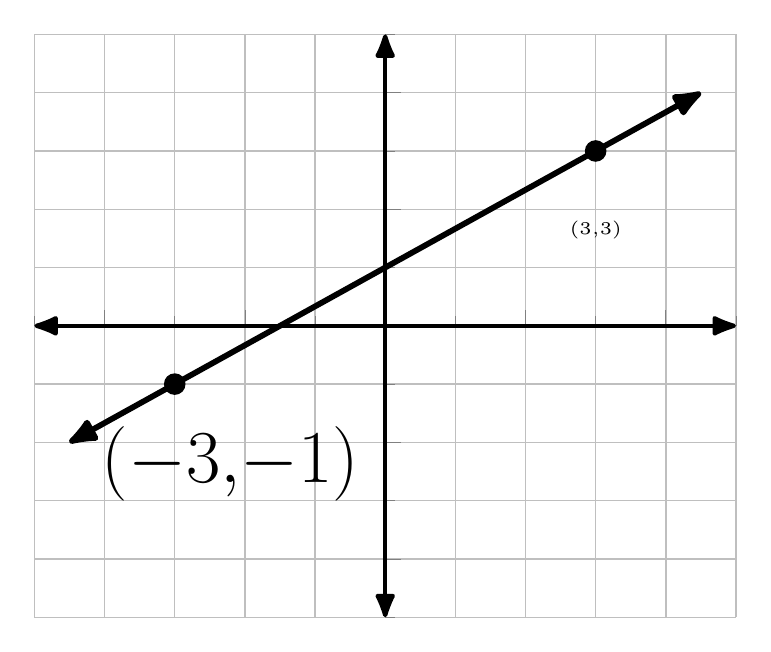
\begin{tikzpicture}[place/.style={circle, fill=black, inner sep=0pt, outer sep=0pt, minimum size=6pt}, scale=1.3
]
\begin{axis} 
[
xticklabels={}, 
yticklabels={}, 
ymin=-5, ymax=5,
xmin=-5, xmax=5,
axis lines = center, 
inner axis line style={Latex[round]-Latex[round],very thick}, 
grid=both,
minor tick num=1, 
%xlabel=$\scriptstyle x$,
%ylabel=$\scriptstyle y$, 
tick align=inside,  
%every axis y label/.style={rotate=0, black, at={(0.5,1.05)},}, 
%every axis x label/.style={rotate=0, black, at={(1.05,0.5)},}, 
%domain=-4.5:4.5, 
%samples=200,
] 

\addplot[<->, >={Latex[round]}, ultra thick, domain=-4.5:4.5, samples=200]{(2/3)*x+1}node[]{};

\node (A) at (-3,-1) [place] {}; 
\node(A-label) at ($(A)+(-55:27pt)$) {\Huge $ \scriptstyle (-3,-1)$};

\node (B) at (3,3) [place] {}; 
\node(B-label) at ($(B)+(-90:22pt)$) {$ \scriptscriptstyle (3,3)$};

\end{axis} 
\end{tikzpicture} 
 
\vspce 
\item \hspce 
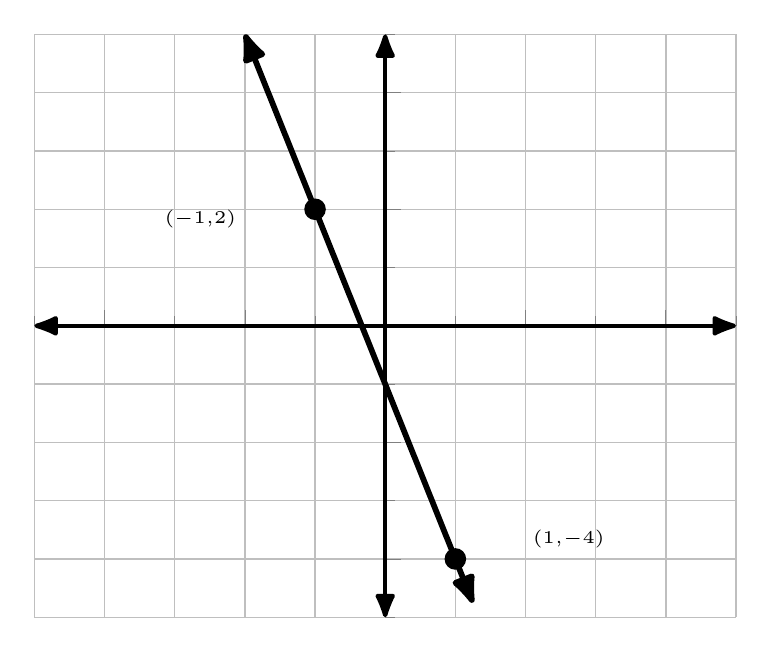
\begin{tikzpicture}[place/.style={circle, fill=black, inner sep=0pt, outer sep=0pt, minimum size=6pt}, scale=1.3
]
\begin{axis} 
[
xticklabels={}, 
yticklabels={}, 
ymin=-5, ymax=5,
xmin=-5, xmax=5,
axis lines = center, 
inner axis line style={Latex[round]-Latex[round],very thick}, 
grid=both,
minor tick num=1, 
%xlabel=$\scriptstyle x$,
%ylabel=$\scriptstyle y$, 
tick align=inside,  
%every axis y label/.style={rotate=0, black, at={(0.5,1.05)},}, 
%every axis x label/.style={rotate=0, black, at={(1.05,0.5)},}, 
%domain=-4.5:4.5, 
%samples=200,
] 

\addplot[<->, >={Latex[round]}, ultra thick, domain=-2:1.25, samples=200]{-3*x-1}node[]{};

\node (A) at (-1,2) [place] {}; 
\node(A-label) at ($(A)+(185:32pt)$) {$ \scriptscriptstyle (-1,2)$};

\node (B) at (1,-4) [place] {}; 
\node(B-label) at ($(B)+(10:32pt)$) {$ \scriptscriptstyle (1,-4)$};

\end{axis} 
\end{tikzpicture} 
 
\vspce 
\item \hspce 
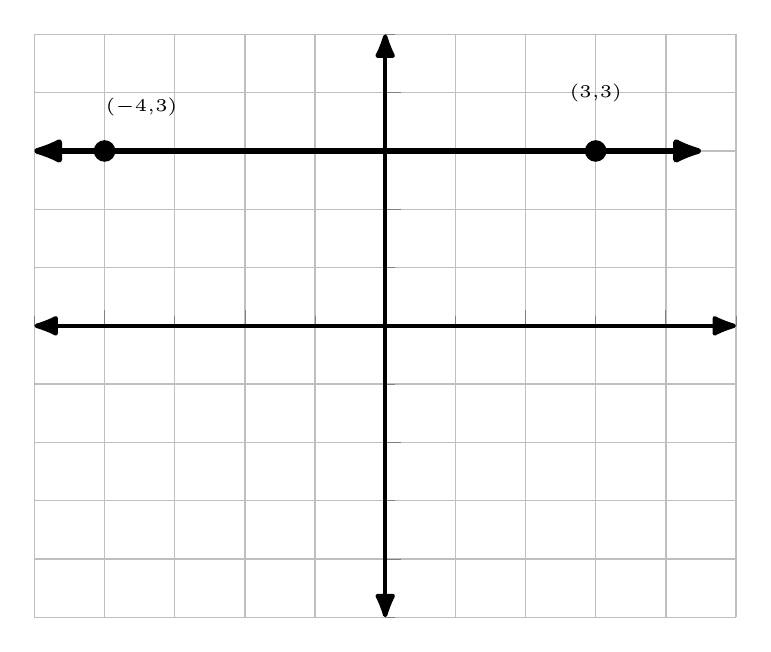
\begin{tikzpicture}[place/.style={circle, fill=black, inner sep=0pt, outer sep=0pt, minimum size=6pt}, scale=1.3
]
\begin{axis} 
[
xticklabels={}, 
yticklabels={}, 
ymin=-5, ymax=5,
xmin=-5, xmax=5,
axis lines = center, 
inner axis line style={Latex[round]-Latex[round],very thick}, 
grid=both,
minor tick num=1, 
%xlabel=$\scriptstyle x$,
%ylabel=$\scriptstyle y$, 
tick align=inside,  
%every axis y label/.style={rotate=0, black, at={(0.5,1.05)},}, 
%every axis x label/.style={rotate=0, black, at={(1.05,0.5)},}, 
%domain=-4.5:4.5, 
%samples=200,
] 

\addplot[<->, >={Latex[round]}, ultra thick, domain=-5:4.5, samples=200]{3}node[]{};

\node (A) at (-4,3) [place] {}; 
\node(A-label) at ($(A)+(50:16pt)$) {$ \scriptscriptstyle (-4,3)$};

\node (B) at (3,3) [place] {}; 
\node(B-label) at ($(B)+(90:16pt)$) {$ \scriptscriptstyle (3,3)$};

\end{axis} 
\end{tikzpicture} 
  
\vspce 
\item \hspce 
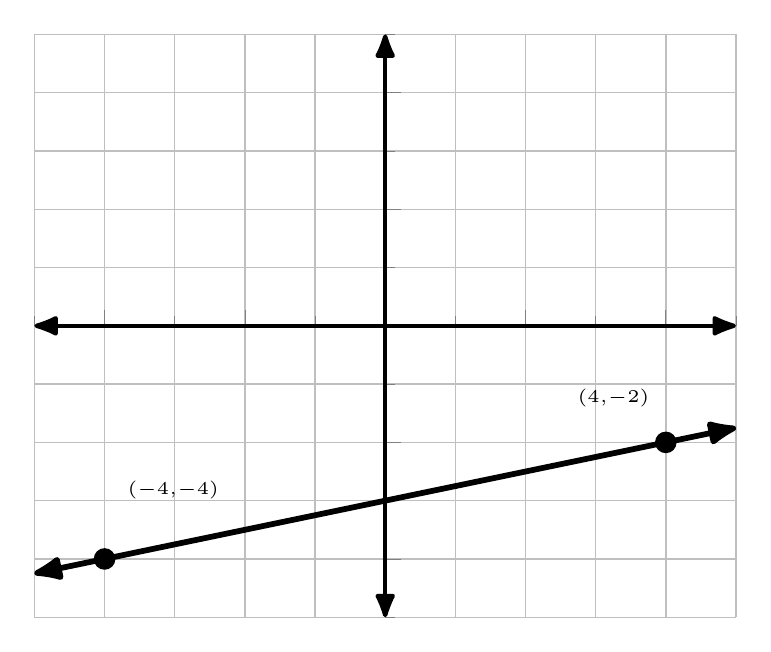
\begin{tikzpicture}[place/.style={circle, fill=black, inner sep=0pt, outer sep=0pt, minimum size=6pt}, scale=1.3
]
\begin{axis} 
[
xticklabels={}, 
yticklabels={}, 
ymin=-5, ymax=5,
xmin=-5, xmax=5,
axis lines = center, 
inner axis line style={Latex[round]-Latex[round],very thick}, 
grid=both,
minor tick num=1, 
%xlabel=$\scriptstyle x$,
%ylabel=$\scriptstyle y$, 
tick align=inside,  
%every axis y label/.style={rotate=0, black, at={(0.5,1.05)},}, 
%every axis x label/.style={rotate=0, black, at={(1.05,0.5)},}, 
%domain=-4.5:4.5, 
%samples=200,
] 

\addplot[<->, >={Latex[round]}, ultra thick, domain=-5:5, samples=200]{x/4-3}node[]{};

\node (A) at (-4,-4) [place] {}; 
\node(A-label) at ($(A)+(45:27pt)$) {$ \scriptscriptstyle (-4,-4)$};

\node (B) at (4,-2) [place] {}; 
\node(B-label) at ($(B)+(140:19pt)$) {$ \scriptscriptstyle (4,-2)$};

\end{axis} 
\end{tikzpicture} 
  
\vspce 
\item \hspce 
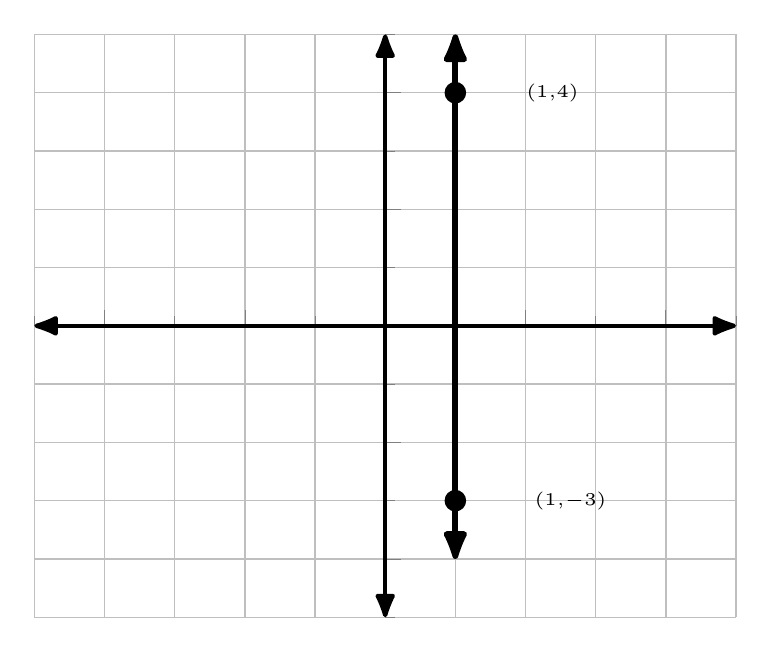
\begin{tikzpicture}[place/.style={circle, fill=black, inner sep=0pt, outer sep=0pt, minimum size=6pt}, scale=1.3
]
\begin{axis} 
[
xticklabels={}, 
yticklabels={}, 
ymin=-5, ymax=5,
xmin=-5, xmax=5,
axis lines = center, 
inner axis line style={Latex[round]-Latex[round],very thick}, 
grid=both,
minor tick num=1, 
%xlabel=$\scriptstyle x$,
%ylabel=$\scriptstyle y$, 
tick align=inside,  
%every axis y label/.style={rotate=0, black, at={(0.5,1.05)},}, 
%every axis x label/.style={rotate=0, black, at={(1.05,0.5)},}, 
%domain=-4.5:4.5, 
%samples=200,
] 

%\addplot[<->, ultra thick, domain=-2.25:0.5, samples=200]{(7/2)*x+3}node[]{};

\node (A) at (1, -3) [place] {}; 
\node(A-label) at ($(A)+(0:32pt)$) {$ \scriptscriptstyle (1, -3)$};

\node (B) at (1, 4) [place] {}; 
\node(B-label) at ($(B)+(0:27pt)$) {$ \scriptscriptstyle (1, 4)$};
\draw[<->, >={Latex[round]}, ultra thick] (1,5) -- (1,-4); 

\end{axis} 
\end{tikzpicture} 
 
\end{multicols} 
\end{enumerate}   

\item  Determine  the slope and trend  of each  line. 

\begin{enumerate}[label = \arabic*. ]
%begin{multicols}{2}

\item \hspce $\ { f(x)=-3x  + 7}$ 
\vspce 
\item \hspce $\ { f(x)=\displaystyle  \frac{1}{4}x-8}$ 
\vspce 
\item \hspce $\ {2x  -  y  = 5 }$ 
\vspce 
\item \hspce $\ { \displaystyle  \frac{1}{2}x+\displaystyle  \frac{1}{4}y-8 = 0 }$ 
\vspce 
\item \hspce $\ {2y  + 1 = 0 }$ 

%end{multicols} 
\end{enumerate}  

\end{enumerate}  
\end{frame}

% frame 2
\vertadjust
\begin{frame} 
%\begin{center}
\textbf{Slope of a Line 
}
\end{center}

\vspce

Slope: the steepness of a line

%\begin{itemize} 
%\item 
The slope $\ {m }$ of a line can be computed by finding the quotient of the rise and the run. \[\ {m=\displaystyle  \frac{rise}{run}}\] 

%\item 
The slope $\ {m }$  of the line passing through two points $\ { P_1(x_1, y_1)}$   and $\ {P_2(x_2, y_2) }$  is given by
\begin{center}
 $\ {m = \displaystyle  \frac{y_2-y_1}{x_2-x_1}}$, where  $\ {x_1 \neq x_2 }$.
\end{center} 
%\item 
The slope of the horizontal line is zero while that of the vertical line is undefined. 
%\item 

The value of the slope $\ {m }$  tells the trend of the graph. 
%\begin{itemize} 
%\item 

If $\ {m }$ is positive, then the graph is increasing from left to right.
%\item 

If $\ {m }$ is negative, then the graph is decreasing from left to right.
%\item 

If $\ {m }$ is zero, then the graph is a horizontal  line.
%\item 

If $\ {m }$ is undefined, then the graph is a vertical line.
%\end{itemize} 

%\end{itemize} 


% \\
%\textbf{Practice Exercises}
%\textbf{Problem Set}

\vspce


%\begin{enumerate}[label = \Alph*. ]
%\item 
\def \scaleforhandout{0.6}

A. Find the slope of each line below. 

\begin{enumerate}[label = \arabic*. ]
\begin{multicols}{2}

\item \hspce 
\begin{tikzpicture}[place/.style={circle, fill=black, inner sep=0pt, outer sep=0pt, minimum size=6pt}, scale=\scaleforhandout %scale=1.3
]
\begin{axis} 
[
xticklabels={}, 
yticklabels={}, 
ymin=-5, ymax=5,
xmin=-5, xmax=5,
axis lines = center, 
inner axis line style={Latex[round]-Latex[round],very thick}, 
grid=both,
minor tick num=1, 
%xlabel=$\scriptstyle x$,
%ylabel=$\scriptstyle y$, 
tick align=inside,  
%every axis y label/.style={rotate=0, black, at={(0.5,1.05)},}, 
%every axis x label/.style={rotate=0, black, at={(1.05,0.5)},}, 
%domain=-4.5:4.5, 
%samples=200,
] 

\addplot[<->, >={Latex[round]},  ultra thick, domain=-2.25:0.5, samples=200]{(7/2)*x+3}node[]{};

\node (A) at (-2,-4) [place] {}; 
\node(A-label) at ($(A)+(135:37pt)$) {\Huge $ \scriptstyle (-2,-4)$};

\node (B) at (0,3) [place] {}; 
\node(B-label) at ($(B)+(5:27pt)$) {$ \scriptscriptstyle (0,3)$};

\end{axis} 
\end{tikzpicture} 
 
\vspce 
\item \hspce 
\begin{tikzpicture}[place/.style={circle, fill=black, inner sep=0pt, outer sep=0pt, minimum size=6pt}, scale=\scaleforhandout %scale=1.3
]
\begin{axis} 
[
xticklabels={}, 
yticklabels={}, 
ymin=-5, ymax=5,
xmin=-5, xmax=5,
axis lines = center, 
inner axis line style={Latex[round]-Latex[round],very thick}, 
grid=both,
minor tick num=1, 
%xlabel=$\scriptstyle x$,
%ylabel=$\scriptstyle y$, 
tick align=inside,  
%every axis y label/.style={rotate=0, black, at={(0.5,1.05)},}, 
%every axis x label/.style={rotate=0, black, at={(1.05,0.5)},}, 
%domain=-4.5:4.5, 
%samples=200,
] 

\addplot[<->, >={Latex[round]}, ultra thick, domain=-1.5:4, samples=200]{-x+3}node[]{};

\node (A) at (0,3) [place] {}; 
\node(A-label) at ($(A)+(185:32pt)$) {$ \scriptscriptstyle (0,3)$};

\node (B) at (2,1) [place] {}; 
\node(B-label) at ($(B)+(20:27pt)$) {$ \scriptscriptstyle (2,1)$};

\end{axis} 
\end{tikzpicture} 
 
\vspce 
\item \hspce 
\begin{tikzpicture}[place/.style={circle, fill=black, inner sep=0pt, outer sep=0pt, minimum size=6pt},scale=\scaleforhandout % scale=1.3
]
\begin{axis} 
[
xticklabels={}, 
yticklabels={}, 
ymin=-5, ymax=5,
xmin=-5, xmax=5,
axis lines = center, 
inner axis line style={Latex[round]-Latex[round],very thick}, 
grid=both,
minor tick num=1, 
%xlabel=$\scriptstyle x$,
%ylabel=$\scriptstyle y$, 
tick align=inside,  
%every axis y label/.style={rotate=0, black, at={(0.5,1.05)},}, 
%every axis x label/.style={rotate=0, black, at={(1.05,0.5)},}, 
%domain=-4.5:4.5, 
%samples=200,
] 

\addplot[<->, >={Latex[round]}, ultra thick, domain=-4.5:4.5, samples=200]{-3}node[]{};

\node (A) at (-3,-3) [place] {}; 
\node(A-label) at ($(A)+(90:17pt)$) {$ \scriptscriptstyle (-3,-3)$};

\node (B) at (2,-3) [place] {}; 
\node(B-label) at ($(B)+(90:17pt)$) {$ \scriptscriptstyle (2,-3)$};

\end{axis} 
\end{tikzpicture} 
  
\vspce 
\item \hspce 
\begin{tikzpicture}[place/.style={circle, fill=black, inner sep=0pt, outer sep=0pt, minimum size=6pt}, scale=\scaleforhandout %scale=1.3
]
\begin{axis} 
[
xticklabels={}, 
yticklabels={}, 
ymin=-5, ymax=5,
xmin=-5, xmax=5,
axis lines = center, 
inner axis line style={Latex[round]-Latex[round],very thick}, 
grid=both,
minor tick num=1, 
%xlabel=$\scriptstyle x$,
%ylabel=$\scriptstyle y$, 
tick align=inside,  
%every axis y label/.style={rotate=0, black, at={(0.5,1.05)},}, 
%every axis x label/.style={rotate=0, black, at={(1.05,0.5)},}, 
%domain=-4.5:4.5, 
%samples=200,
] 

\addplot[<->, >={Latex[round]}, ultra thick, domain=-4:5, samples=200]{x/2-2}node[]{};

\node (A) at (0,-2) [place] {}; 
\node(A-label) at ($(A)+(165:32pt)$) {$ \scriptscriptstyle (0,-2)$};

\node (B) at (4,0) [place] {}; 
\node(B-label) at ($(B)+(130:22pt)$) {$ \scriptscriptstyle (4,0)$};

\end{axis} 
\end{tikzpicture} 
  
\vspce 
\item \hspce 
\begin{tikzpicture}[place/.style={circle, fill=black, inner sep=0pt, outer sep=0pt, minimum size=6pt}, scale=\scaleforhandout %scale=1.3
]
\begin{axis} 
[
xticklabels={}, 
yticklabels={}, 
ymin=-5, ymax=5,
xmin=-5, xmax=5,
axis lines = center, 
inner axis line style={Latex[round]-Latex[round],very thick}, 
grid=both,
minor tick num=1, 
%xlabel=$\scriptstyle x$,
%ylabel=$\scriptstyle y$, 
tick align=inside,  
%every axis y label/.style={rotate=0, black, at={(0.5,1.05)},}, 
%every axis x label/.style={rotate=0, black, at={(1.05,0.5)},}, 
%domain=-4.5:4.5, 
%samples=200,
] 

%\addplot[<->, ultra thick, domain=-2.25:0.5, samples=200]{(7/2)*x+3}node[]{};

\node (A) at (-2, -4) [place] {}; 
\node(A-label) at ($(A)+(180:32pt)$) {\huge $ \scriptstyle (-2,-4)$};

\node (B) at (-2, 3) [place] {}; 
\node(B-label) at ($(B)+(180:32pt)$) {\Huge $ \scriptstyle (-2,3)$};
\draw[<->, >={Latex[round]},ultra thick] (-2,-5) -- (-2,4); 

\end{axis} 
\end{tikzpicture} 
 
\end{multicols} 
\end{enumerate}   




%\end{enumerate} 


B. Determine  the slope and trend  of each  line. 

\begin{enumerate}[label = \arabic*. ]
%begin{multicols}{2}

\item \hspce $\ { f(x)=2x-5}$ 
%\vspce 
\item \hspce $\ { f(x)=x+6}$ 
%\vspce 
\item \hspce $\ { f(x) =\displaystyle  \frac{2}{3}x-\displaystyle  \frac{1}{2} }$ 
%\vspce 
\item \hspce $\ { 7x-3y-10 = 0 }$ 
%\vspce 
\item \hspce $\ {x  = 8 }$ 

%end{multicols} 
\end{enumerate}  
%\textbf{Practice Exercises}
\textbf{Problem Set}

\vspce
\def \scaleforhandout{0.6}

%\begin{enumerate}[label = \Alph*. ]
%\item 
A. Find the slope of each line below. 

\begin{enumerate}[label = \arabic*. ]
\begin{multicols}{2}

\item \hspce 
\begin{tikzpicture}[place/.style={circle, fill=black, inner sep=0pt, outer sep=0pt, minimum size=6pt}, scale=\scaleforhandout
]
\begin{axis} 
[
xticklabels={}, 
yticklabels={}, 
ymin=-5, ymax=5,
xmin=-5, xmax=5,
axis lines = center, 
inner axis line style={Latex[round]-Latex[round],very thick}, 
grid=both,
minor tick num=1, 
%xlabel=$\scriptstyle x$,
%ylabel=$\scriptstyle y$, 
tick align=inside,  
%every axis y label/.style={rotate=0, black, at={(0.5,1.05)},}, 
%every axis x label/.style={rotate=0, black, at={(1.05,0.5)},}, 
%domain=-4.5:4.5, 
%samples=200,
] 

\addplot[<->, >={Latex[round]}, ultra thick, domain=-4.5:4.5, samples=200]{(2/3)*x+1}node[]{};

\node (A) at (-3,-1) [place] {}; 
\node(A-label) at ($(A)+(-55:27pt)$) {\Huge $ \scriptstyle (-3,-1)$};

\node (B) at (3,3) [place] {}; 
\node(B-label) at ($(B)+(-90:22pt)$) {\huge$(3,3)$};

\end{axis} 
\end{tikzpicture} 
 
\vspce 
\item \hspce 
\begin{tikzpicture}[place/.style={circle, fill=black, inner sep=0pt, outer sep=0pt, minimum size=6pt}, scale=\scaleforhandout
]
\begin{axis} 
[
xticklabels={}, 
yticklabels={}, 
ymin=-5, ymax=5,
xmin=-5, xmax=5,
axis lines = center, 
inner axis line style={Latex[round]-Latex[round],very thick}, 
grid=both,
minor tick num=1, 
%xlabel=$\scriptstyle x$,
%ylabel=$\scriptstyle y$, 
tick align=inside,  
%every axis y label/.style={rotate=0, black, at={(0.5,1.05)},}, 
%every axis x label/.style={rotate=0, black, at={(1.05,0.5)},}, 
%domain=-4.5:4.5, 
%samples=200,
] 

\addplot[<->, >={Latex[round]}, ultra thick, domain=-2:1.25, samples=200]{-3*x-1}node[]{};

\node (A) at (-1,2) [place] {}; 
\node(A-label) at ($(A)+(185:32pt)$) {\huge$(-1,2)$};

\node (B) at (1,-4) [place] {}; 
\node(B-label) at ($(B)+(10:32pt)$) {\huge$(1,-4)$};

\end{axis} 
\end{tikzpicture} 
 
\vspce 
\item \hspce 
\begin{tikzpicture}[place/.style={circle, fill=black, inner sep=0pt, outer sep=0pt, minimum size=6pt}, scale=\scaleforhandout
]
\begin{axis} 
[
xticklabels={}, 
yticklabels={}, 
ymin=-5, ymax=5,
xmin=-5, xmax=5,
axis lines = center, 
inner axis line style={Latex[round]-Latex[round],very thick}, 
grid=both,
minor tick num=1, 
%xlabel=$\scriptstyle x$,
%ylabel=$\scriptstyle y$, 
tick align=inside,  
%every axis y label/.style={rotate=0, black, at={(0.5,1.05)},}, 
%every axis x label/.style={rotate=0, black, at={(1.05,0.5)},}, 
%domain=-4.5:4.5, 
%samples=200,
] 

\addplot[<->, >={Latex[round]}, ultra thick, domain=-5:4.5, samples=200]{3}node[]{};

\node (A) at (-4,3) [place] {}; 
\node(A-label) at ($(A)+(50:16pt)$) {\huge$(-4,3)$};

\node (B) at (3,3) [place] {}; 
\node(B-label) at ($(B)+(90:16pt)$) {\huge$(3,3)$};

\end{axis} 
\end{tikzpicture} 
  
\vspce 
\item \hspce 
\begin{tikzpicture}[place/.style={circle, fill=black, inner sep=0pt, outer sep=0pt, minimum size=6pt}, scale=\scaleforhandout
]
\begin{axis} 
[
xticklabels={}, 
yticklabels={}, 
ymin=-5, ymax=5,
xmin=-5, xmax=5,
axis lines = center, 
inner axis line style={Latex[round]-Latex[round],very thick}, 
grid=both,
minor tick num=1, 
%xlabel=$\scriptstyle x$,
%ylabel=$\scriptstyle y$, 
tick align=inside,  
%every axis y label/.style={rotate=0, black, at={(0.5,1.05)},}, 
%every axis x label/.style={rotate=0, black, at={(1.05,0.5)},}, 
%domain=-4.5:4.5, 
%samples=200,
] 

\addplot[<->, >={Latex[round]}, ultra thick, domain=-5:5, samples=200]{x/4-3}node[]{};

\node (A) at (-4,-4) [place] {}; 
\node(A-label) at ($(A)+(45:27pt)$) {\huge$(-4,-4)$};

\node (B) at (4,-2) [place] {}; 
\node(B-label) at ($(B)+(140:19pt)$) {\huge$(4,-2)$};

\end{axis} 
\end{tikzpicture} 
  
\vspce 
\item \hspce 
\begin{tikzpicture}[place/.style={circle, fill=black, inner sep=0pt, outer sep=0pt, minimum size=6pt}, scale=\scaleforhandout
]
\begin{axis} 
[
xticklabels={}, 
yticklabels={}, 
ymin=-5, ymax=5,
xmin=-5, xmax=5,
axis lines = center, 
inner axis line style={Latex[round]-Latex[round],very thick}, 
grid=both,
minor tick num=1, 
%xlabel=$\scriptstyle x$,
%ylabel=$\scriptstyle y$, 
tick align=inside,  
%every axis y label/.style={rotate=0, black, at={(0.5,1.05)},}, 
%every axis x label/.style={rotate=0, black, at={(1.05,0.5)},}, 
%domain=-4.5:4.5, 
%samples=200,
] 

%\addplot[<->, ultra thick, domain=-2.25:0.5, samples=200]{(7/2)*x+3}node[]{};

\node (A) at (1, -3) [place] {}; 
\node(A-label) at ($(A)+(0:32pt)$) {\huge$(1, -3)$};

\node (B) at (1, 4) [place] {}; 
\node(B-label) at ($(B)+(0:27pt)$) {\huge$(1, 4)$};
\draw[<->, >={Latex[round]}, ultra thick] (1,5) -- (1,-4); 

\end{axis} 
\end{tikzpicture} 
 
\end{multicols} 
\end{enumerate}   

%\item  
B. Determine  the slope and trend  of each  line. 

\begin{enumerate}[label = \arabic*. ]
%begin{multicols}{2}

\item \hspce $\ { f(x)=-3x  + 7}$ 
\vspce 
\item \hspce $\ { f(x)=\displaystyle  \frac{1}{4}x-8}$ 
\vspce 
\item \hspce $\ {2x  -  y  = 5 }$ 
\vspce 
\item \hspce $\ { \displaystyle  \frac{1}{2}x+\displaystyle  \frac{1}{4}y-8 = 0 }$ 
\vspce 
\item \hspce $\ {2y  + 1 = 0 }$ 

%end{multicols} 
\end{enumerate}  

%\end{enumerate}  
%%\textbf{Practice Exercises}
\textbf{Problem Set}

\vspce


\begin{enumerate}[label = \Alph*. ]
\item Find the slope of each line below. 

\begin{enumerate}[label = \arabic*. ]
\begin{multicols}{2}

\item \hspce 
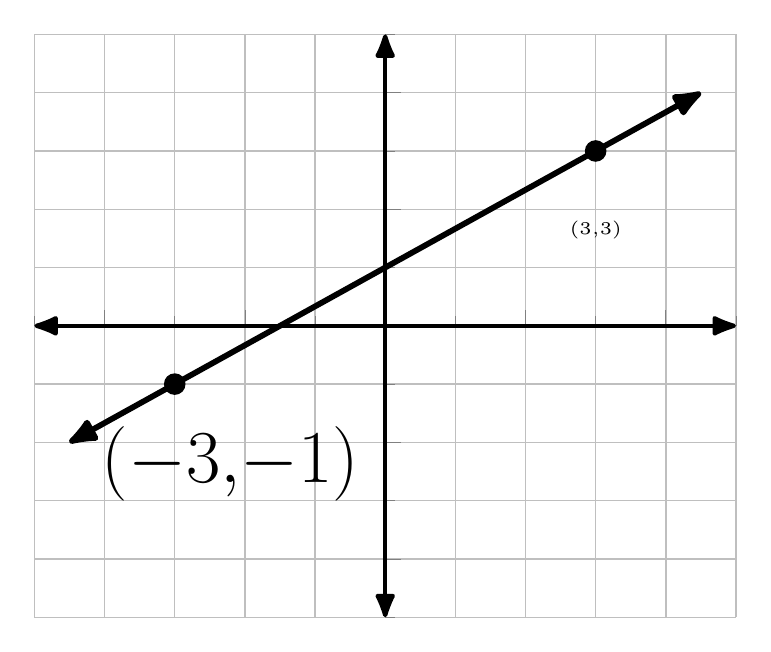
\begin{tikzpicture}[place/.style={circle, fill=black, inner sep=0pt, outer sep=0pt, minimum size=6pt}, scale=1.3
]
\begin{axis} 
[
xticklabels={}, 
yticklabels={}, 
ymin=-5, ymax=5,
xmin=-5, xmax=5,
axis lines = center, 
inner axis line style={Latex[round]-Latex[round],very thick}, 
grid=both,
minor tick num=1, 
%xlabel=$\scriptstyle x$,
%ylabel=$\scriptstyle y$, 
tick align=inside,  
%every axis y label/.style={rotate=0, black, at={(0.5,1.05)},}, 
%every axis x label/.style={rotate=0, black, at={(1.05,0.5)},}, 
%domain=-4.5:4.5, 
%samples=200,
] 

\addplot[<->, >={Latex[round]}, ultra thick, domain=-4.5:4.5, samples=200]{(2/3)*x+1}node[]{};

\node (A) at (-3,-1) [place] {}; 
\node(A-label) at ($(A)+(-55:27pt)$) {\Huge $ \scriptstyle (-3,-1)$};

\node (B) at (3,3) [place] {}; 
\node(B-label) at ($(B)+(-90:22pt)$) {$ \scriptscriptstyle (3,3)$};

\end{axis} 
\end{tikzpicture} 
 
\vspce 
\item \hspce 
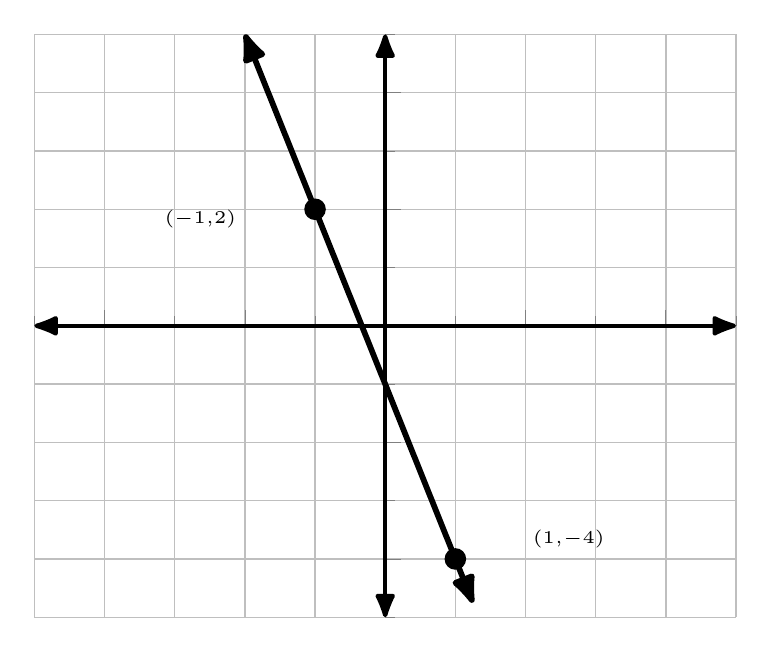
\begin{tikzpicture}[place/.style={circle, fill=black, inner sep=0pt, outer sep=0pt, minimum size=6pt}, scale=1.3
]
\begin{axis} 
[
xticklabels={}, 
yticklabels={}, 
ymin=-5, ymax=5,
xmin=-5, xmax=5,
axis lines = center, 
inner axis line style={Latex[round]-Latex[round],very thick}, 
grid=both,
minor tick num=1, 
%xlabel=$\scriptstyle x$,
%ylabel=$\scriptstyle y$, 
tick align=inside,  
%every axis y label/.style={rotate=0, black, at={(0.5,1.05)},}, 
%every axis x label/.style={rotate=0, black, at={(1.05,0.5)},}, 
%domain=-4.5:4.5, 
%samples=200,
] 

\addplot[<->, >={Latex[round]}, ultra thick, domain=-2:1.25, samples=200]{-3*x-1}node[]{};

\node (A) at (-1,2) [place] {}; 
\node(A-label) at ($(A)+(185:32pt)$) {$ \scriptscriptstyle (-1,2)$};

\node (B) at (1,-4) [place] {}; 
\node(B-label) at ($(B)+(10:32pt)$) {$ \scriptscriptstyle (1,-4)$};

\end{axis} 
\end{tikzpicture} 
 
\vspce 
\item \hspce 
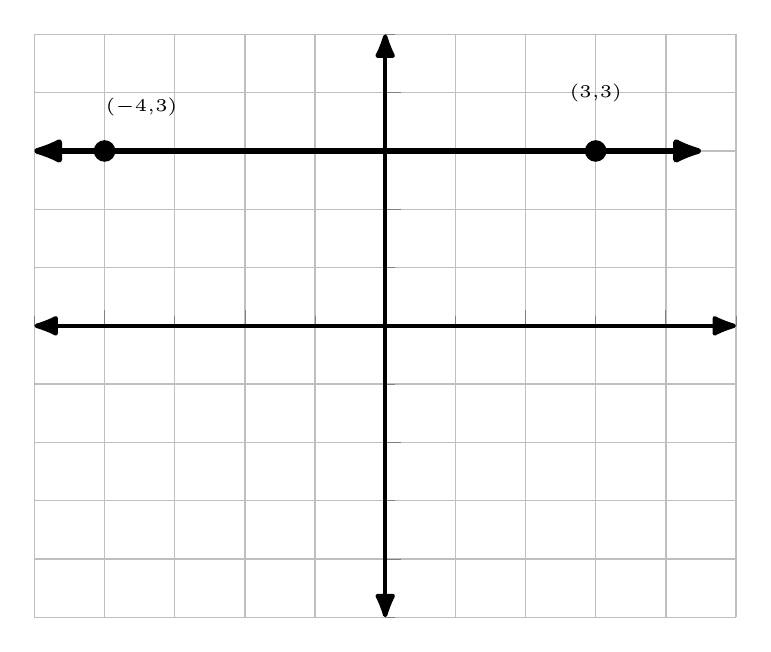
\begin{tikzpicture}[place/.style={circle, fill=black, inner sep=0pt, outer sep=0pt, minimum size=6pt}, scale=1.3
]
\begin{axis} 
[
xticklabels={}, 
yticklabels={}, 
ymin=-5, ymax=5,
xmin=-5, xmax=5,
axis lines = center, 
inner axis line style={Latex[round]-Latex[round],very thick}, 
grid=both,
minor tick num=1, 
%xlabel=$\scriptstyle x$,
%ylabel=$\scriptstyle y$, 
tick align=inside,  
%every axis y label/.style={rotate=0, black, at={(0.5,1.05)},}, 
%every axis x label/.style={rotate=0, black, at={(1.05,0.5)},}, 
%domain=-4.5:4.5, 
%samples=200,
] 

\addplot[<->, >={Latex[round]}, ultra thick, domain=-5:4.5, samples=200]{3}node[]{};

\node (A) at (-4,3) [place] {}; 
\node(A-label) at ($(A)+(50:16pt)$) {$ \scriptscriptstyle (-4,3)$};

\node (B) at (3,3) [place] {}; 
\node(B-label) at ($(B)+(90:16pt)$) {$ \scriptscriptstyle (3,3)$};

\end{axis} 
\end{tikzpicture} 
  
\vspce 
\item \hspce 
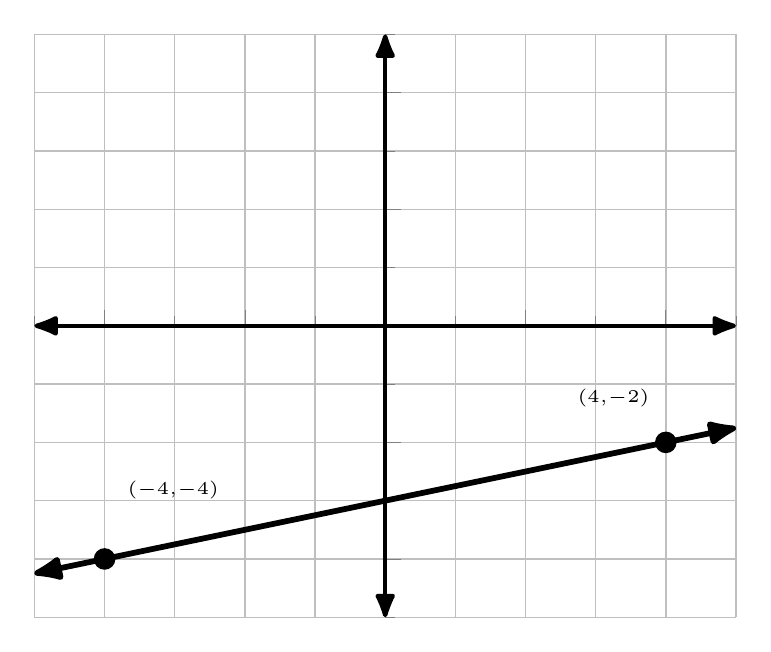
\begin{tikzpicture}[place/.style={circle, fill=black, inner sep=0pt, outer sep=0pt, minimum size=6pt}, scale=1.3
]
\begin{axis} 
[
xticklabels={}, 
yticklabels={}, 
ymin=-5, ymax=5,
xmin=-5, xmax=5,
axis lines = center, 
inner axis line style={Latex[round]-Latex[round],very thick}, 
grid=both,
minor tick num=1, 
%xlabel=$\scriptstyle x$,
%ylabel=$\scriptstyle y$, 
tick align=inside,  
%every axis y label/.style={rotate=0, black, at={(0.5,1.05)},}, 
%every axis x label/.style={rotate=0, black, at={(1.05,0.5)},}, 
%domain=-4.5:4.5, 
%samples=200,
] 

\addplot[<->, >={Latex[round]}, ultra thick, domain=-5:5, samples=200]{x/4-3}node[]{};

\node (A) at (-4,-4) [place] {}; 
\node(A-label) at ($(A)+(45:27pt)$) {$ \scriptscriptstyle (-4,-4)$};

\node (B) at (4,-2) [place] {}; 
\node(B-label) at ($(B)+(140:19pt)$) {$ \scriptscriptstyle (4,-2)$};

\end{axis} 
\end{tikzpicture} 
  
\vspce 
\item \hspce 
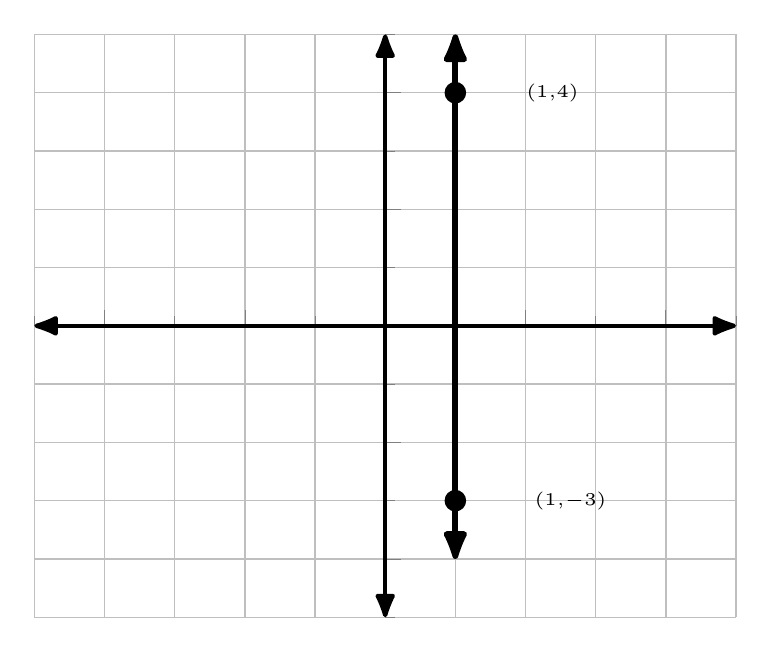
\begin{tikzpicture}[place/.style={circle, fill=black, inner sep=0pt, outer sep=0pt, minimum size=6pt}, scale=1.3
]
\begin{axis} 
[
xticklabels={}, 
yticklabels={}, 
ymin=-5, ymax=5,
xmin=-5, xmax=5,
axis lines = center, 
inner axis line style={Latex[round]-Latex[round],very thick}, 
grid=both,
minor tick num=1, 
%xlabel=$\scriptstyle x$,
%ylabel=$\scriptstyle y$, 
tick align=inside,  
%every axis y label/.style={rotate=0, black, at={(0.5,1.05)},}, 
%every axis x label/.style={rotate=0, black, at={(1.05,0.5)},}, 
%domain=-4.5:4.5, 
%samples=200,
] 

%\addplot[<->, ultra thick, domain=-2.25:0.5, samples=200]{(7/2)*x+3}node[]{};

\node (A) at (1, -3) [place] {}; 
\node(A-label) at ($(A)+(0:32pt)$) {$ \scriptscriptstyle (1, -3)$};

\node (B) at (1, 4) [place] {}; 
\node(B-label) at ($(B)+(0:27pt)$) {$ \scriptscriptstyle (1, 4)$};
\draw[<->, >={Latex[round]}, ultra thick] (1,5) -- (1,-4); 

\end{axis} 
\end{tikzpicture} 
 
\end{multicols} 
\end{enumerate}   

\item  Determine  the slope and trend  of each  line. 

\begin{enumerate}[label = \arabic*. ]
%begin{multicols}{2}

\item \hspce $\ { f(x)=-3x  + 7}$ 
\vspce 
\item \hspce $\ { f(x)=\displaystyle  \frac{1}{4}x-8}$ 
\vspce 
\item \hspce $\ {2x  -  y  = 5 }$ 
\vspce 
\item \hspce $\ { \displaystyle  \frac{1}{2}x+\displaystyle  \frac{1}{4}y-8 = 0 }$ 
\vspce 
\item \hspce $\ {2y  + 1 = 0 }$ 

%end{multicols} 
\end{enumerate}  

\end{enumerate}  
\end{frame}

% frame 3
\vertadjustb
\begin{frame} 
\begin{center}
\textbf{Slope of a Line 
}
\end{center}

\vspce

Slope: the steepness of a line

%\begin{itemize} 
%\item 
The slope $\ {m }$ of a line can be computed by finding the quotient of the rise and the run. \[\ {m=\displaystyle  \frac{rise}{run}}\] 

%\item 
The slope $\ {m }$  of the line passing through two points $\ { P_1(x_1, y_1)}$   and $\ {P_2(x_2, y_2) }$  is given by
\begin{center}
 $\ {m = \displaystyle  \frac{y_2-y_1}{x_2-x_1}}$, where  $\ {x_1 \neq x_2 }$.
\end{center} 
%\item 
The slope of the horizontal line is zero while that of the vertical line is undefined. 
%\item 

The value of the slope $\ {m }$  tells the trend of the graph. 
%\begin{itemize} 
%\item 

If $\ {m }$ is positive, then the graph is increasing from left to right.
%\item 

If $\ {m }$ is negative, then the graph is decreasing from left to right.
%\item 

If $\ {m }$ is zero, then the graph is a horizontal  line.
%\item 

If $\ {m }$ is undefined, then the graph is a vertical line.
%\end{itemize} 

%\end{itemize} 


 %\\
\textbf{Practice Exercises}
%\textbf{Problem Set}

\vspce


%\begin{enumerate}[label = \Alph*. ]
%\item 
\def \scaleforhandout{0.6}

A. Find the slope of each line below. 

\begin{enumerate}[label = \arabic*. ]
\begin{multicols}{2}

\item \hspce 
\begin{tikzpicture}[place/.style={circle, fill=black, inner sep=0pt, outer sep=0pt, minimum size=6pt}, scale=\scaleforhandout %scale=1.3
]
\begin{axis} 
[
xticklabels={}, 
yticklabels={}, 
ymin=-5, ymax=5,
xmin=-5, xmax=5,
axis lines = center, 
inner axis line style={Latex[round]-Latex[round],very thick}, 
grid=both,
minor tick num=1, 
%xlabel=$\scriptstyle x$,
%ylabel=$\scriptstyle y$, 
tick align=inside,  
%every axis y label/.style={rotate=0, black, at={(0.5,1.05)},}, 
%every axis x label/.style={rotate=0, black, at={(1.05,0.5)},}, 
%domain=-4.5:4.5, 
%samples=200,
] 

\addplot[<->, >={Latex[round]},  ultra thick, domain=-2.25:0.5, samples=200]{(7/2)*x+3}node[]{};

\node (A) at (-2,-4) [place] {}; 
\node(A-label) at ($(A)+(135:37pt)$) {\Huge $ \scriptstyle (-2,-4)$};

\node (B) at (0,3) [place] {}; 
\node(B-label) at ($(B)+(5:27pt)$) {\huge $ (0,3)$};

\end{axis} 
\end{tikzpicture} 
 
\vspce 
\item \hspce 
\begin{tikzpicture}[place/.style={circle, fill=black, inner sep=0pt, outer sep=0pt, minimum size=6pt}, scale=\scaleforhandout %scale=1.3
]
\begin{axis} 
[
xticklabels={}, 
yticklabels={}, 
ymin=-5, ymax=5,
xmin=-5, xmax=5,
axis lines = center, 
inner axis line style={Latex[round]-Latex[round],very thick}, 
grid=both,
minor tick num=1, 
%xlabel=$\scriptstyle x$,
%ylabel=$\scriptstyle y$, 
tick align=inside,  
%every axis y label/.style={rotate=0, black, at={(0.5,1.05)},}, 
%every axis x label/.style={rotate=0, black, at={(1.05,0.5)},}, 
%domain=-4.5:4.5, 
%samples=200,
] 

\addplot[<->, >={Latex[round]}, ultra thick, domain=-1.5:4, samples=200]{-x+3}node[]{};

\node (A) at (0,3) [place] {}; 
\node(A-label) at ($(A)+(185:32pt)$) {\huge $(0,3)$};

\node (B) at (2,1) [place] {}; 
\node(B-label) at ($(B)+(20:27pt)$) {\huge$(2,1)$};

\end{axis} 
\end{tikzpicture} 
 
\vspce 
\item \hspce 
\begin{tikzpicture}[place/.style={circle, fill=black, inner sep=0pt, outer sep=0pt, minimum size=6pt},scale=\scaleforhandout % scale=1.3
]
\begin{axis} 
[
xticklabels={}, 
yticklabels={}, 
ymin=-5, ymax=5,
xmin=-5, xmax=5,
axis lines = center, 
inner axis line style={Latex[round]-Latex[round],very thick}, 
grid=both,
minor tick num=1, 
%xlabel=$\scriptstyle x$,
%ylabel=$\scriptstyle y$, 
tick align=inside,  
%every axis y label/.style={rotate=0, black, at={(0.5,1.05)},}, 
%every axis x label/.style={rotate=0, black, at={(1.05,0.5)},}, 
%domain=-4.5:4.5, 
%samples=200,
] 

\addplot[<->, >={Latex[round]}, ultra thick, domain=-4.5:4.5, samples=200]{-3}node[]{};

\node (A) at (-3,-3) [place] {}; 
\node(A-label) at ($(A)+(90:17pt)$) {\huge$(-3,-3)$};

\node (B) at (2,-3) [place] {}; 
\node(B-label) at ($(B)+(90:17pt)$) {\huge$(2,-3)$};

\end{axis} 
\end{tikzpicture} 
  
\vspce 
\item \hspce 
\begin{tikzpicture}[place/.style={circle, fill=black, inner sep=0pt, outer sep=0pt, minimum size=6pt}, scale=\scaleforhandout %scale=1.3
]
\begin{axis} 
[
xticklabels={}, 
yticklabels={}, 
ymin=-5, ymax=5,
xmin=-5, xmax=5,
axis lines = center, 
inner axis line style={Latex[round]-Latex[round],very thick}, 
grid=both,
minor tick num=1, 
%xlabel=$\scriptstyle x$,
%ylabel=$\scriptstyle y$, 
tick align=inside,  
%every axis y label/.style={rotate=0, black, at={(0.5,1.05)},}, 
%every axis x label/.style={rotate=0, black, at={(1.05,0.5)},}, 
%domain=-4.5:4.5, 
%samples=200,
] 

\addplot[<->, >={Latex[round]}, ultra thick, domain=-4:5, samples=200]{x/2-2}node[]{};

\node (A) at (0,-2) [place] {}; 
\node(A-label) at ($(A)+(165:32pt)$) {\huge$(0,-2)$};

\node (B) at (4,0) [place] {}; 
\node(B-label) at ($(B)+(130:22pt)$) {\huge$(4,0)$};

\end{axis} 
\end{tikzpicture} 
  
\vspce 
\item \hspce 
\begin{tikzpicture}[place/.style={circle, fill=black, inner sep=0pt, outer sep=0pt, minimum size=6pt}, scale=\scaleforhandout %scale=1.3
]
\begin{axis} 
[
xticklabels={}, 
yticklabels={}, 
ymin=-5, ymax=5,
xmin=-5, xmax=5,
axis lines = center, 
inner axis line style={Latex[round]-Latex[round],very thick}, 
grid=both,
minor tick num=1, 
%xlabel=$\scriptstyle x$,
%ylabel=$\scriptstyle y$, 
tick align=inside,  
%every axis y label/.style={rotate=0, black, at={(0.5,1.05)},}, 
%every axis x label/.style={rotate=0, black, at={(1.05,0.5)},}, 
%domain=-4.5:4.5, 
%samples=200,
] 

%\addplot[<->, ultra thick, domain=-2.25:0.5, samples=200]{(7/2)*x+3}node[]{};

\node (A) at (-2, -4) [place] {}; 
\node(A-label) at ($(A)+(180:32pt)$) {\huge $ \scriptstyle (-2,-4)$};

\node (B) at (-2, 3) [place] {}; 
\node(B-label) at ($(B)+(180:32pt)$) {\Huge $ \scriptstyle (-2,3)$};
\draw[<->, >={Latex[round]},ultra thick] (-2,-5) -- (-2,4); 

\end{axis} 
\end{tikzpicture} 
 
\end{multicols} 
\end{enumerate}   




%\end{enumerate} 


%B. Determine  the slope and trend  of each  line. 

\begin{enumerate}[label = \arabic*. ]
%begin{multicols}{2}

\item \hspce $\ { f(x)=2x-5}$ 
%\vspce 
\item \hspce $\ { f(x)=x+6}$ 
%\vspce 
\item \hspce $\ { f(x) =\displaystyle  \frac{2}{3}x-\displaystyle  \frac{1}{2} }$ 
%\vspce 
\item \hspce $\ { 7x-3y-10 = 0 }$ 
%\vspce 
\item \hspce $\ {x  = 8 }$ 

%end{multicols} 
\end{enumerate}  
%%\textbf{Practice Exercises}
\textbf{Problem Set}

\vspce


\begin{enumerate}[label = \Alph*. ]
\item Find the slope of each line below. 

\begin{enumerate}[label = \arabic*. ]
\begin{multicols}{2}

\item \hspce 
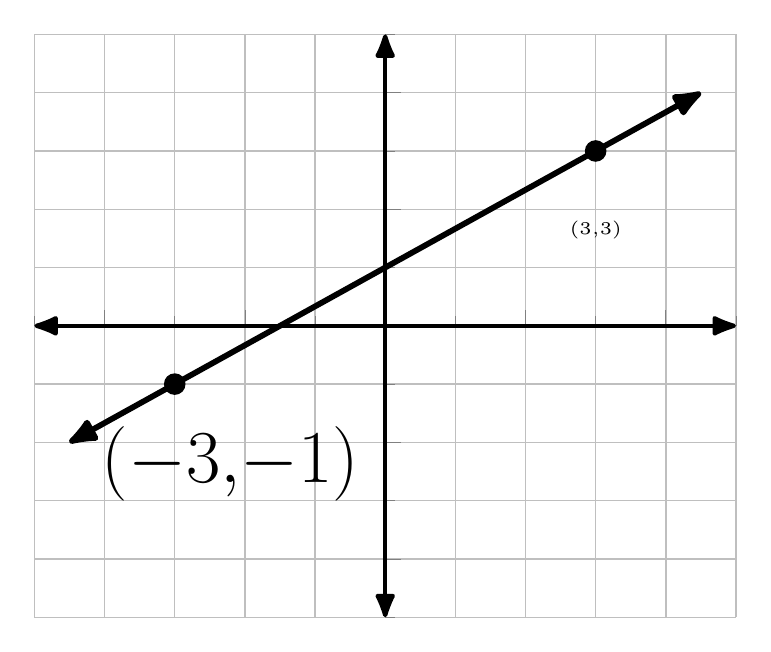
\begin{tikzpicture}[place/.style={circle, fill=black, inner sep=0pt, outer sep=0pt, minimum size=6pt}, scale=1.3
]
\begin{axis} 
[
xticklabels={}, 
yticklabels={}, 
ymin=-5, ymax=5,
xmin=-5, xmax=5,
axis lines = center, 
inner axis line style={Latex[round]-Latex[round],very thick}, 
grid=both,
minor tick num=1, 
%xlabel=$\scriptstyle x$,
%ylabel=$\scriptstyle y$, 
tick align=inside,  
%every axis y label/.style={rotate=0, black, at={(0.5,1.05)},}, 
%every axis x label/.style={rotate=0, black, at={(1.05,0.5)},}, 
%domain=-4.5:4.5, 
%samples=200,
] 

\addplot[<->, >={Latex[round]}, ultra thick, domain=-4.5:4.5, samples=200]{(2/3)*x+1}node[]{};

\node (A) at (-3,-1) [place] {}; 
\node(A-label) at ($(A)+(-55:27pt)$) {\Huge $ \scriptstyle (-3,-1)$};

\node (B) at (3,3) [place] {}; 
\node(B-label) at ($(B)+(-90:22pt)$) {$ \scriptscriptstyle (3,3)$};

\end{axis} 
\end{tikzpicture} 
 
\vspce 
\item \hspce 
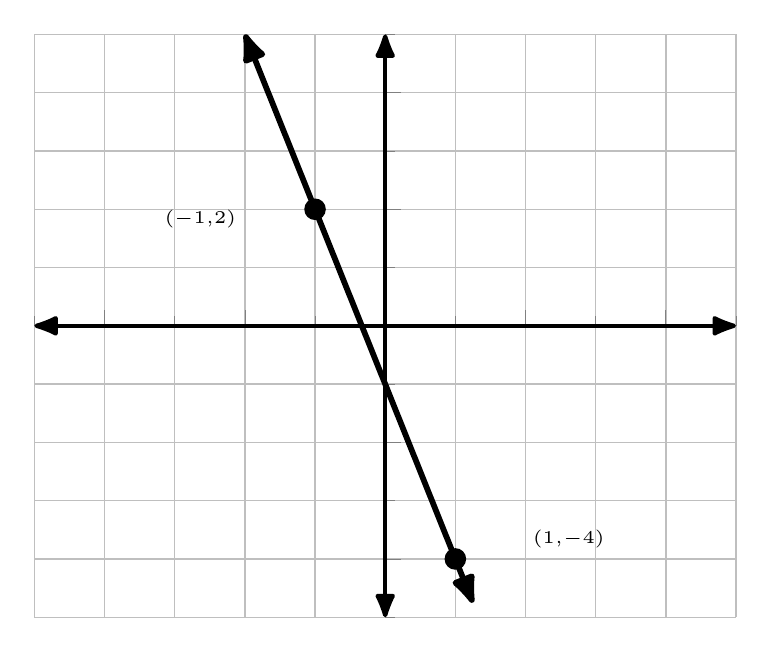
\begin{tikzpicture}[place/.style={circle, fill=black, inner sep=0pt, outer sep=0pt, minimum size=6pt}, scale=1.3
]
\begin{axis} 
[
xticklabels={}, 
yticklabels={}, 
ymin=-5, ymax=5,
xmin=-5, xmax=5,
axis lines = center, 
inner axis line style={Latex[round]-Latex[round],very thick}, 
grid=both,
minor tick num=1, 
%xlabel=$\scriptstyle x$,
%ylabel=$\scriptstyle y$, 
tick align=inside,  
%every axis y label/.style={rotate=0, black, at={(0.5,1.05)},}, 
%every axis x label/.style={rotate=0, black, at={(1.05,0.5)},}, 
%domain=-4.5:4.5, 
%samples=200,
] 

\addplot[<->, >={Latex[round]}, ultra thick, domain=-2:1.25, samples=200]{-3*x-1}node[]{};

\node (A) at (-1,2) [place] {}; 
\node(A-label) at ($(A)+(185:32pt)$) {$ \scriptscriptstyle (-1,2)$};

\node (B) at (1,-4) [place] {}; 
\node(B-label) at ($(B)+(10:32pt)$) {$ \scriptscriptstyle (1,-4)$};

\end{axis} 
\end{tikzpicture} 
 
\vspce 
\item \hspce 
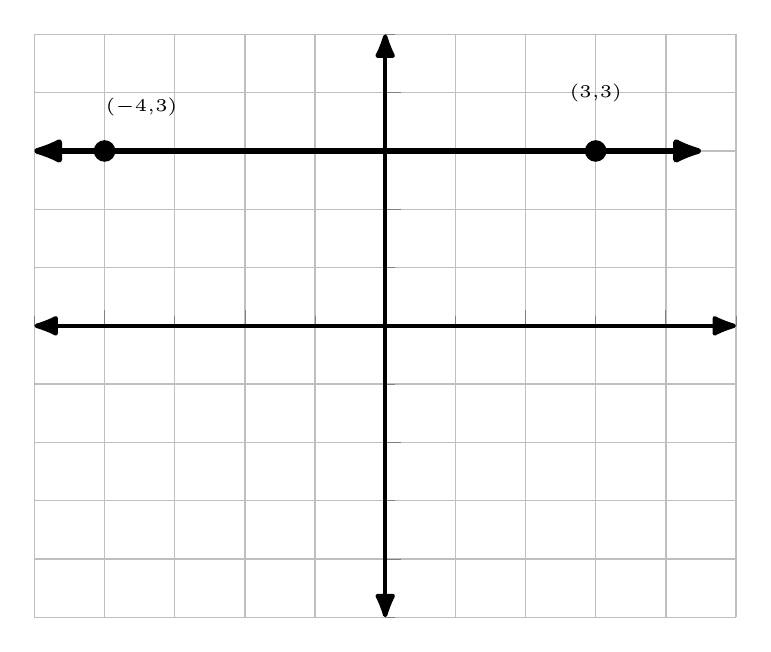
\begin{tikzpicture}[place/.style={circle, fill=black, inner sep=0pt, outer sep=0pt, minimum size=6pt}, scale=1.3
]
\begin{axis} 
[
xticklabels={}, 
yticklabels={}, 
ymin=-5, ymax=5,
xmin=-5, xmax=5,
axis lines = center, 
inner axis line style={Latex[round]-Latex[round],very thick}, 
grid=both,
minor tick num=1, 
%xlabel=$\scriptstyle x$,
%ylabel=$\scriptstyle y$, 
tick align=inside,  
%every axis y label/.style={rotate=0, black, at={(0.5,1.05)},}, 
%every axis x label/.style={rotate=0, black, at={(1.05,0.5)},}, 
%domain=-4.5:4.5, 
%samples=200,
] 

\addplot[<->, >={Latex[round]}, ultra thick, domain=-5:4.5, samples=200]{3}node[]{};

\node (A) at (-4,3) [place] {}; 
\node(A-label) at ($(A)+(50:16pt)$) {$ \scriptscriptstyle (-4,3)$};

\node (B) at (3,3) [place] {}; 
\node(B-label) at ($(B)+(90:16pt)$) {$ \scriptscriptstyle (3,3)$};

\end{axis} 
\end{tikzpicture} 
  
\vspce 
\item \hspce 
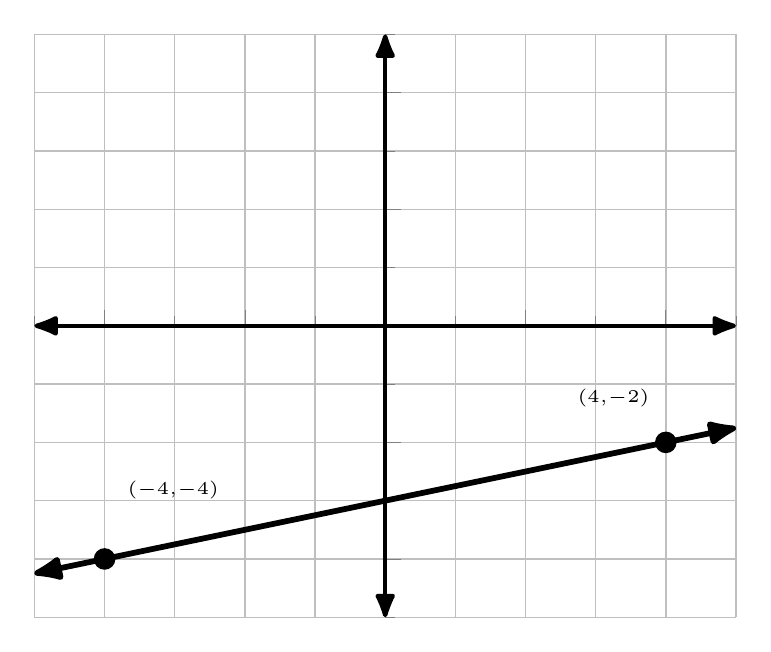
\begin{tikzpicture}[place/.style={circle, fill=black, inner sep=0pt, outer sep=0pt, minimum size=6pt}, scale=1.3
]
\begin{axis} 
[
xticklabels={}, 
yticklabels={}, 
ymin=-5, ymax=5,
xmin=-5, xmax=5,
axis lines = center, 
inner axis line style={Latex[round]-Latex[round],very thick}, 
grid=both,
minor tick num=1, 
%xlabel=$\scriptstyle x$,
%ylabel=$\scriptstyle y$, 
tick align=inside,  
%every axis y label/.style={rotate=0, black, at={(0.5,1.05)},}, 
%every axis x label/.style={rotate=0, black, at={(1.05,0.5)},}, 
%domain=-4.5:4.5, 
%samples=200,
] 

\addplot[<->, >={Latex[round]}, ultra thick, domain=-5:5, samples=200]{x/4-3}node[]{};

\node (A) at (-4,-4) [place] {}; 
\node(A-label) at ($(A)+(45:27pt)$) {$ \scriptscriptstyle (-4,-4)$};

\node (B) at (4,-2) [place] {}; 
\node(B-label) at ($(B)+(140:19pt)$) {$ \scriptscriptstyle (4,-2)$};

\end{axis} 
\end{tikzpicture} 
  
\vspce 
\item \hspce 
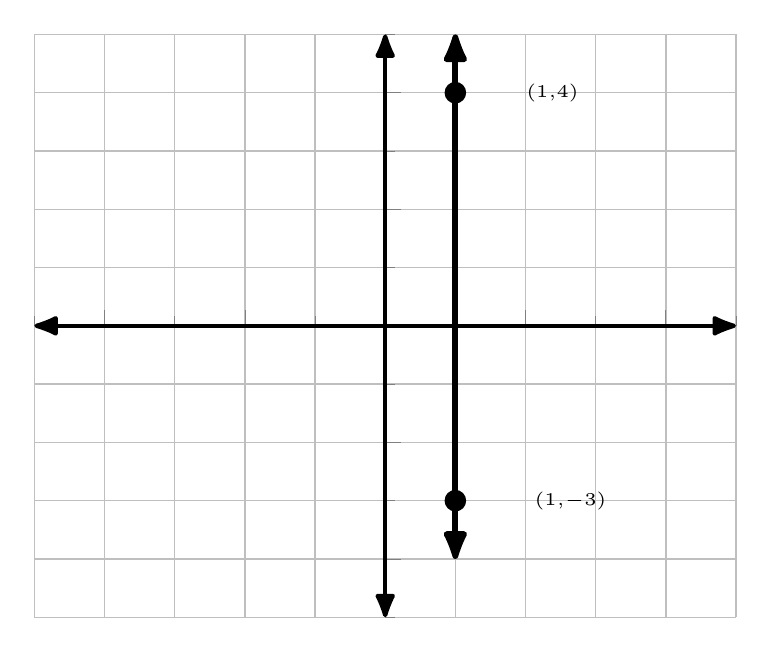
\begin{tikzpicture}[place/.style={circle, fill=black, inner sep=0pt, outer sep=0pt, minimum size=6pt}, scale=1.3
]
\begin{axis} 
[
xticklabels={}, 
yticklabels={}, 
ymin=-5, ymax=5,
xmin=-5, xmax=5,
axis lines = center, 
inner axis line style={Latex[round]-Latex[round],very thick}, 
grid=both,
minor tick num=1, 
%xlabel=$\scriptstyle x$,
%ylabel=$\scriptstyle y$, 
tick align=inside,  
%every axis y label/.style={rotate=0, black, at={(0.5,1.05)},}, 
%every axis x label/.style={rotate=0, black, at={(1.05,0.5)},}, 
%domain=-4.5:4.5, 
%samples=200,
] 

%\addplot[<->, ultra thick, domain=-2.25:0.5, samples=200]{(7/2)*x+3}node[]{};

\node (A) at (1, -3) [place] {}; 
\node(A-label) at ($(A)+(0:32pt)$) {$ \scriptscriptstyle (1, -3)$};

\node (B) at (1, 4) [place] {}; 
\node(B-label) at ($(B)+(0:27pt)$) {$ \scriptscriptstyle (1, 4)$};
\draw[<->, >={Latex[round]}, ultra thick] (1,5) -- (1,-4); 

\end{axis} 
\end{tikzpicture} 
 
\end{multicols} 
\end{enumerate}   

\item  Determine  the slope and trend  of each  line. 

\begin{enumerate}[label = \arabic*. ]
%begin{multicols}{2}

\item \hspce $\ { f(x)=-3x  + 7}$ 
\vspce 
\item \hspce $\ { f(x)=\displaystyle  \frac{1}{4}x-8}$ 
\vspce 
\item \hspce $\ {2x  -  y  = 5 }$ 
\vspce 
\item \hspce $\ { \displaystyle  \frac{1}{2}x+\displaystyle  \frac{1}{4}y-8 = 0 }$ 
\vspce 
\item \hspce $\ {2y  + 1 = 0 }$ 

%end{multicols} 
\end{enumerate}  

\end{enumerate}  
\end{frame}

% frame 4
\vertadjustb
\begin{frame} 
%\begin{center}
\textbf{Slope of a Line 
}
\end{center}

\vspce

Slope: the steepness of a line

%\begin{itemize} 
%\item 
The slope $\ {m }$ of a line can be computed by finding the quotient of the rise and the run. \[\ {m=\displaystyle  \frac{rise}{run}}\] 

%\item 
The slope $\ {m }$  of the line passing through two points $\ { P_1(x_1, y_1)}$   and $\ {P_2(x_2, y_2) }$  is given by
\begin{center}
 $\ {m = \displaystyle  \frac{y_2-y_1}{x_2-x_1}}$, where  $\ {x_1 \neq x_2 }$.
\end{center} 
%\item 
The slope of the horizontal line is zero while that of the vertical line is undefined. 
%\item 

The value of the slope $\ {m }$  tells the trend of the graph. 
%\begin{itemize} 
%\item 

If $\ {m }$ is positive, then the graph is increasing from left to right.
%\item 

If $\ {m }$ is negative, then the graph is decreasing from left to right.
%\item 

If $\ {m }$ is zero, then the graph is a horizontal  line.
%\item 

If $\ {m }$ is undefined, then the graph is a vertical line.
%\end{itemize} 

%\end{itemize} 


% \\
%\textbf{Practice Exercises}
%\textbf{Problem Set}

\vspce


%\begin{enumerate}[label = \Alph*. ]
%\item 
\def \scaleforhandout{0.6}

A. Find the slope of each line below. 

\begin{enumerate}[label = \arabic*. ]
\begin{multicols}{2}

\item \hspce 
\begin{tikzpicture}[place/.style={circle, fill=black, inner sep=0pt, outer sep=0pt, minimum size=6pt}, scale=\scaleforhandout %scale=1.3
]
\begin{axis} 
[
xticklabels={}, 
yticklabels={}, 
ymin=-5, ymax=5,
xmin=-5, xmax=5,
axis lines = center, 
inner axis line style={Latex[round]-Latex[round],very thick}, 
grid=both,
minor tick num=1, 
%xlabel=$\scriptstyle x$,
%ylabel=$\scriptstyle y$, 
tick align=inside,  
%every axis y label/.style={rotate=0, black, at={(0.5,1.05)},}, 
%every axis x label/.style={rotate=0, black, at={(1.05,0.5)},}, 
%domain=-4.5:4.5, 
%samples=200,
] 

\addplot[<->, >={Latex[round]},  ultra thick, domain=-2.25:0.5, samples=200]{(7/2)*x+3}node[]{};

\node (A) at (-2,-4) [place] {}; 
\node(A-label) at ($(A)+(135:37pt)$) {\Huge $ \scriptstyle (-2,-4)$};

\node (B) at (0,3) [place] {}; 
\node(B-label) at ($(B)+(5:27pt)$) {$ \scriptscriptstyle (0,3)$};

\end{axis} 
\end{tikzpicture} 
 
\vspce 
\item \hspce 
\begin{tikzpicture}[place/.style={circle, fill=black, inner sep=0pt, outer sep=0pt, minimum size=6pt}, scale=\scaleforhandout %scale=1.3
]
\begin{axis} 
[
xticklabels={}, 
yticklabels={}, 
ymin=-5, ymax=5,
xmin=-5, xmax=5,
axis lines = center, 
inner axis line style={Latex[round]-Latex[round],very thick}, 
grid=both,
minor tick num=1, 
%xlabel=$\scriptstyle x$,
%ylabel=$\scriptstyle y$, 
tick align=inside,  
%every axis y label/.style={rotate=0, black, at={(0.5,1.05)},}, 
%every axis x label/.style={rotate=0, black, at={(1.05,0.5)},}, 
%domain=-4.5:4.5, 
%samples=200,
] 

\addplot[<->, >={Latex[round]}, ultra thick, domain=-1.5:4, samples=200]{-x+3}node[]{};

\node (A) at (0,3) [place] {}; 
\node(A-label) at ($(A)+(185:32pt)$) {$ \scriptscriptstyle (0,3)$};

\node (B) at (2,1) [place] {}; 
\node(B-label) at ($(B)+(20:27pt)$) {$ \scriptscriptstyle (2,1)$};

\end{axis} 
\end{tikzpicture} 
 
\vspce 
\item \hspce 
\begin{tikzpicture}[place/.style={circle, fill=black, inner sep=0pt, outer sep=0pt, minimum size=6pt},scale=\scaleforhandout % scale=1.3
]
\begin{axis} 
[
xticklabels={}, 
yticklabels={}, 
ymin=-5, ymax=5,
xmin=-5, xmax=5,
axis lines = center, 
inner axis line style={Latex[round]-Latex[round],very thick}, 
grid=both,
minor tick num=1, 
%xlabel=$\scriptstyle x$,
%ylabel=$\scriptstyle y$, 
tick align=inside,  
%every axis y label/.style={rotate=0, black, at={(0.5,1.05)},}, 
%every axis x label/.style={rotate=0, black, at={(1.05,0.5)},}, 
%domain=-4.5:4.5, 
%samples=200,
] 

\addplot[<->, >={Latex[round]}, ultra thick, domain=-4.5:4.5, samples=200]{-3}node[]{};

\node (A) at (-3,-3) [place] {}; 
\node(A-label) at ($(A)+(90:17pt)$) {$ \scriptscriptstyle (-3,-3)$};

\node (B) at (2,-3) [place] {}; 
\node(B-label) at ($(B)+(90:17pt)$) {$ \scriptscriptstyle (2,-3)$};

\end{axis} 
\end{tikzpicture} 
  
\vspce 
\item \hspce 
\begin{tikzpicture}[place/.style={circle, fill=black, inner sep=0pt, outer sep=0pt, minimum size=6pt}, scale=\scaleforhandout %scale=1.3
]
\begin{axis} 
[
xticklabels={}, 
yticklabels={}, 
ymin=-5, ymax=5,
xmin=-5, xmax=5,
axis lines = center, 
inner axis line style={Latex[round]-Latex[round],very thick}, 
grid=both,
minor tick num=1, 
%xlabel=$\scriptstyle x$,
%ylabel=$\scriptstyle y$, 
tick align=inside,  
%every axis y label/.style={rotate=0, black, at={(0.5,1.05)},}, 
%every axis x label/.style={rotate=0, black, at={(1.05,0.5)},}, 
%domain=-4.5:4.5, 
%samples=200,
] 

\addplot[<->, >={Latex[round]}, ultra thick, domain=-4:5, samples=200]{x/2-2}node[]{};

\node (A) at (0,-2) [place] {}; 
\node(A-label) at ($(A)+(165:32pt)$) {$ \scriptscriptstyle (0,-2)$};

\node (B) at (4,0) [place] {}; 
\node(B-label) at ($(B)+(130:22pt)$) {$ \scriptscriptstyle (4,0)$};

\end{axis} 
\end{tikzpicture} 
  
\vspce 
\item \hspce 
\begin{tikzpicture}[place/.style={circle, fill=black, inner sep=0pt, outer sep=0pt, minimum size=6pt}, scale=\scaleforhandout %scale=1.3
]
\begin{axis} 
[
xticklabels={}, 
yticklabels={}, 
ymin=-5, ymax=5,
xmin=-5, xmax=5,
axis lines = center, 
inner axis line style={Latex[round]-Latex[round],very thick}, 
grid=both,
minor tick num=1, 
%xlabel=$\scriptstyle x$,
%ylabel=$\scriptstyle y$, 
tick align=inside,  
%every axis y label/.style={rotate=0, black, at={(0.5,1.05)},}, 
%every axis x label/.style={rotate=0, black, at={(1.05,0.5)},}, 
%domain=-4.5:4.5, 
%samples=200,
] 

%\addplot[<->, ultra thick, domain=-2.25:0.5, samples=200]{(7/2)*x+3}node[]{};

\node (A) at (-2, -4) [place] {}; 
\node(A-label) at ($(A)+(180:32pt)$) {\huge $ \scriptstyle (-2,-4)$};

\node (B) at (-2, 3) [place] {}; 
\node(B-label) at ($(B)+(180:32pt)$) {\Huge $ \scriptstyle (-2,3)$};
\draw[<->, >={Latex[round]},ultra thick] (-2,-5) -- (-2,4); 

\end{axis} 
\end{tikzpicture} 
 
\end{multicols} 
\end{enumerate}   




%\end{enumerate} 


B. Determine  the slope and trend  of each  line. 

\begin{enumerate}[label = \arabic*. ]
%begin{multicols}{2}

\item \hspce $\ { f(x)=2x-5}$ 
%\vspce 
\item \hspce $\ { f(x)=x+6}$ 
%\vspce 
\item \hspce $\ { f(x) =\displaystyle  \frac{2}{3}x-\displaystyle  \frac{1}{2} }$ 
%\vspce 
\item \hspce $\ { 7x-3y-10 = 0 }$ 
%\vspce 
\item \hspce $\ {x  = 8 }$ 

%end{multicols} 
\end{enumerate}  
%\textbf{Practice Exercises}
\textbf{Problem Set}

\vspce
\def \scaleforhandout{0.6}

%\begin{enumerate}[label = \Alph*. ]
%\item 
A. Find the slope of each line below. 

\begin{enumerate}[label = \arabic*. ]
\begin{multicols}{2}

\item \hspce 
\begin{tikzpicture}[place/.style={circle, fill=black, inner sep=0pt, outer sep=0pt, minimum size=6pt}, scale=\scaleforhandout
]
\begin{axis} 
[
xticklabels={}, 
yticklabels={}, 
ymin=-5, ymax=5,
xmin=-5, xmax=5,
axis lines = center, 
inner axis line style={Latex[round]-Latex[round],very thick}, 
grid=both,
minor tick num=1, 
%xlabel=$\scriptstyle x$,
%ylabel=$\scriptstyle y$, 
tick align=inside,  
%every axis y label/.style={rotate=0, black, at={(0.5,1.05)},}, 
%every axis x label/.style={rotate=0, black, at={(1.05,0.5)},}, 
%domain=-4.5:4.5, 
%samples=200,
] 

\addplot[<->, >={Latex[round]}, ultra thick, domain=-4.5:4.5, samples=200]{(2/3)*x+1}node[]{};

\node (A) at (-3,-1) [place] {}; 
\node(A-label) at ($(A)+(-55:27pt)$) {\Huge $ \scriptstyle (-3,-1)$};

\node (B) at (3,3) [place] {}; 
\node(B-label) at ($(B)+(-90:22pt)$) {\huge$(3,3)$};

\end{axis} 
\end{tikzpicture} 
 
\vspce 
\item \hspce 
\begin{tikzpicture}[place/.style={circle, fill=black, inner sep=0pt, outer sep=0pt, minimum size=6pt}, scale=\scaleforhandout
]
\begin{axis} 
[
xticklabels={}, 
yticklabels={}, 
ymin=-5, ymax=5,
xmin=-5, xmax=5,
axis lines = center, 
inner axis line style={Latex[round]-Latex[round],very thick}, 
grid=both,
minor tick num=1, 
%xlabel=$\scriptstyle x$,
%ylabel=$\scriptstyle y$, 
tick align=inside,  
%every axis y label/.style={rotate=0, black, at={(0.5,1.05)},}, 
%every axis x label/.style={rotate=0, black, at={(1.05,0.5)},}, 
%domain=-4.5:4.5, 
%samples=200,
] 

\addplot[<->, >={Latex[round]}, ultra thick, domain=-2:1.25, samples=200]{-3*x-1}node[]{};

\node (A) at (-1,2) [place] {}; 
\node(A-label) at ($(A)+(185:32pt)$) {\huge$(-1,2)$};

\node (B) at (1,-4) [place] {}; 
\node(B-label) at ($(B)+(10:32pt)$) {\huge$(1,-4)$};

\end{axis} 
\end{tikzpicture} 
 
\vspce 
\item \hspce 
\begin{tikzpicture}[place/.style={circle, fill=black, inner sep=0pt, outer sep=0pt, minimum size=6pt}, scale=\scaleforhandout
]
\begin{axis} 
[
xticklabels={}, 
yticklabels={}, 
ymin=-5, ymax=5,
xmin=-5, xmax=5,
axis lines = center, 
inner axis line style={Latex[round]-Latex[round],very thick}, 
grid=both,
minor tick num=1, 
%xlabel=$\scriptstyle x$,
%ylabel=$\scriptstyle y$, 
tick align=inside,  
%every axis y label/.style={rotate=0, black, at={(0.5,1.05)},}, 
%every axis x label/.style={rotate=0, black, at={(1.05,0.5)},}, 
%domain=-4.5:4.5, 
%samples=200,
] 

\addplot[<->, >={Latex[round]}, ultra thick, domain=-5:4.5, samples=200]{3}node[]{};

\node (A) at (-4,3) [place] {}; 
\node(A-label) at ($(A)+(50:16pt)$) {\huge$(-4,3)$};

\node (B) at (3,3) [place] {}; 
\node(B-label) at ($(B)+(90:16pt)$) {\huge$(3,3)$};

\end{axis} 
\end{tikzpicture} 
  
\vspce 
\item \hspce 
\begin{tikzpicture}[place/.style={circle, fill=black, inner sep=0pt, outer sep=0pt, minimum size=6pt}, scale=\scaleforhandout
]
\begin{axis} 
[
xticklabels={}, 
yticklabels={}, 
ymin=-5, ymax=5,
xmin=-5, xmax=5,
axis lines = center, 
inner axis line style={Latex[round]-Latex[round],very thick}, 
grid=both,
minor tick num=1, 
%xlabel=$\scriptstyle x$,
%ylabel=$\scriptstyle y$, 
tick align=inside,  
%every axis y label/.style={rotate=0, black, at={(0.5,1.05)},}, 
%every axis x label/.style={rotate=0, black, at={(1.05,0.5)},}, 
%domain=-4.5:4.5, 
%samples=200,
] 

\addplot[<->, >={Latex[round]}, ultra thick, domain=-5:5, samples=200]{x/4-3}node[]{};

\node (A) at (-4,-4) [place] {}; 
\node(A-label) at ($(A)+(45:27pt)$) {\huge$(-4,-4)$};

\node (B) at (4,-2) [place] {}; 
\node(B-label) at ($(B)+(140:19pt)$) {\huge$(4,-2)$};

\end{axis} 
\end{tikzpicture} 
  
\vspce 
\item \hspce 
\begin{tikzpicture}[place/.style={circle, fill=black, inner sep=0pt, outer sep=0pt, minimum size=6pt}, scale=\scaleforhandout
]
\begin{axis} 
[
xticklabels={}, 
yticklabels={}, 
ymin=-5, ymax=5,
xmin=-5, xmax=5,
axis lines = center, 
inner axis line style={Latex[round]-Latex[round],very thick}, 
grid=both,
minor tick num=1, 
%xlabel=$\scriptstyle x$,
%ylabel=$\scriptstyle y$, 
tick align=inside,  
%every axis y label/.style={rotate=0, black, at={(0.5,1.05)},}, 
%every axis x label/.style={rotate=0, black, at={(1.05,0.5)},}, 
%domain=-4.5:4.5, 
%samples=200,
] 

%\addplot[<->, ultra thick, domain=-2.25:0.5, samples=200]{(7/2)*x+3}node[]{};

\node (A) at (1, -3) [place] {}; 
\node(A-label) at ($(A)+(0:32pt)$) {\huge$(1, -3)$};

\node (B) at (1, 4) [place] {}; 
\node(B-label) at ($(B)+(0:27pt)$) {\huge$(1, 4)$};
\draw[<->, >={Latex[round]}, ultra thick] (1,5) -- (1,-4); 

\end{axis} 
\end{tikzpicture} 
 
\end{multicols} 
\end{enumerate}   

%\item  
B. Determine  the slope and trend  of each  line. 

\begin{enumerate}[label = \arabic*. ]
%begin{multicols}{2}

\item \hspce $\ { f(x)=-3x  + 7}$ 
\vspce 
\item \hspce $\ { f(x)=\displaystyle  \frac{1}{4}x-8}$ 
\vspce 
\item \hspce $\ {2x  -  y  = 5 }$ 
\vspce 
\item \hspce $\ { \displaystyle  \frac{1}{2}x+\displaystyle  \frac{1}{4}y-8 = 0 }$ 
\vspce 
\item \hspce $\ {2y  + 1 = 0 }$ 

%end{multicols} 
\end{enumerate}  

%\end{enumerate}  
%%\textbf{Practice Exercises}
\textbf{Problem Set}

\vspce


\begin{enumerate}[label = \Alph*. ]
\item Find the slope of each line below. 

\begin{enumerate}[label = \arabic*. ]
\begin{multicols}{2}

\item \hspce 
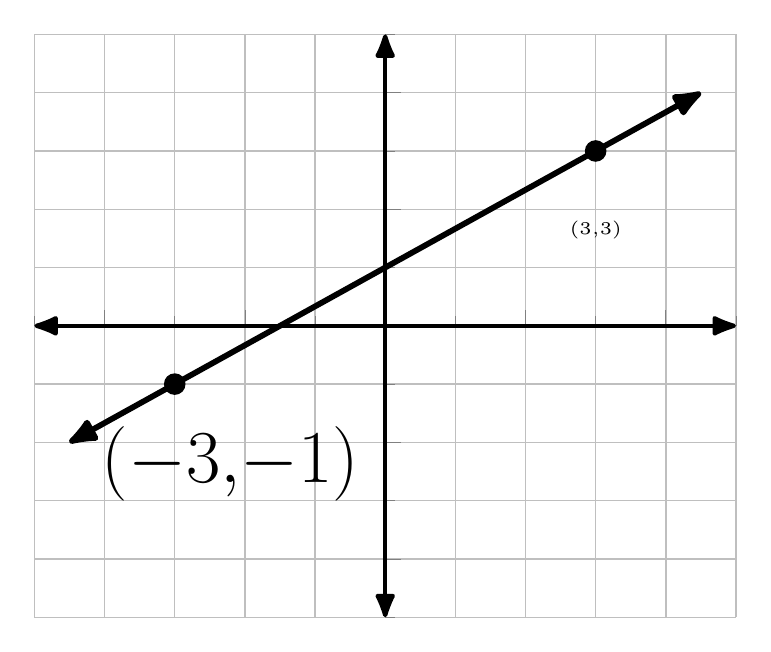
\begin{tikzpicture}[place/.style={circle, fill=black, inner sep=0pt, outer sep=0pt, minimum size=6pt}, scale=1.3
]
\begin{axis} 
[
xticklabels={}, 
yticklabels={}, 
ymin=-5, ymax=5,
xmin=-5, xmax=5,
axis lines = center, 
inner axis line style={Latex[round]-Latex[round],very thick}, 
grid=both,
minor tick num=1, 
%xlabel=$\scriptstyle x$,
%ylabel=$\scriptstyle y$, 
tick align=inside,  
%every axis y label/.style={rotate=0, black, at={(0.5,1.05)},}, 
%every axis x label/.style={rotate=0, black, at={(1.05,0.5)},}, 
%domain=-4.5:4.5, 
%samples=200,
] 

\addplot[<->, >={Latex[round]}, ultra thick, domain=-4.5:4.5, samples=200]{(2/3)*x+1}node[]{};

\node (A) at (-3,-1) [place] {}; 
\node(A-label) at ($(A)+(-55:27pt)$) {\Huge $ \scriptstyle (-3,-1)$};

\node (B) at (3,3) [place] {}; 
\node(B-label) at ($(B)+(-90:22pt)$) {$ \scriptscriptstyle (3,3)$};

\end{axis} 
\end{tikzpicture} 
 
\vspce 
\item \hspce 
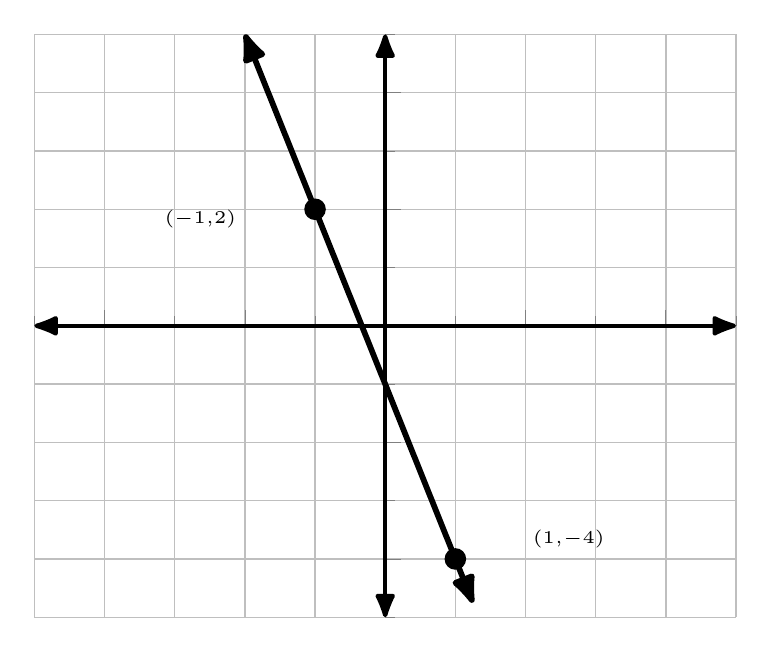
\begin{tikzpicture}[place/.style={circle, fill=black, inner sep=0pt, outer sep=0pt, minimum size=6pt}, scale=1.3
]
\begin{axis} 
[
xticklabels={}, 
yticklabels={}, 
ymin=-5, ymax=5,
xmin=-5, xmax=5,
axis lines = center, 
inner axis line style={Latex[round]-Latex[round],very thick}, 
grid=both,
minor tick num=1, 
%xlabel=$\scriptstyle x$,
%ylabel=$\scriptstyle y$, 
tick align=inside,  
%every axis y label/.style={rotate=0, black, at={(0.5,1.05)},}, 
%every axis x label/.style={rotate=0, black, at={(1.05,0.5)},}, 
%domain=-4.5:4.5, 
%samples=200,
] 

\addplot[<->, >={Latex[round]}, ultra thick, domain=-2:1.25, samples=200]{-3*x-1}node[]{};

\node (A) at (-1,2) [place] {}; 
\node(A-label) at ($(A)+(185:32pt)$) {$ \scriptscriptstyle (-1,2)$};

\node (B) at (1,-4) [place] {}; 
\node(B-label) at ($(B)+(10:32pt)$) {$ \scriptscriptstyle (1,-4)$};

\end{axis} 
\end{tikzpicture} 
 
\vspce 
\item \hspce 
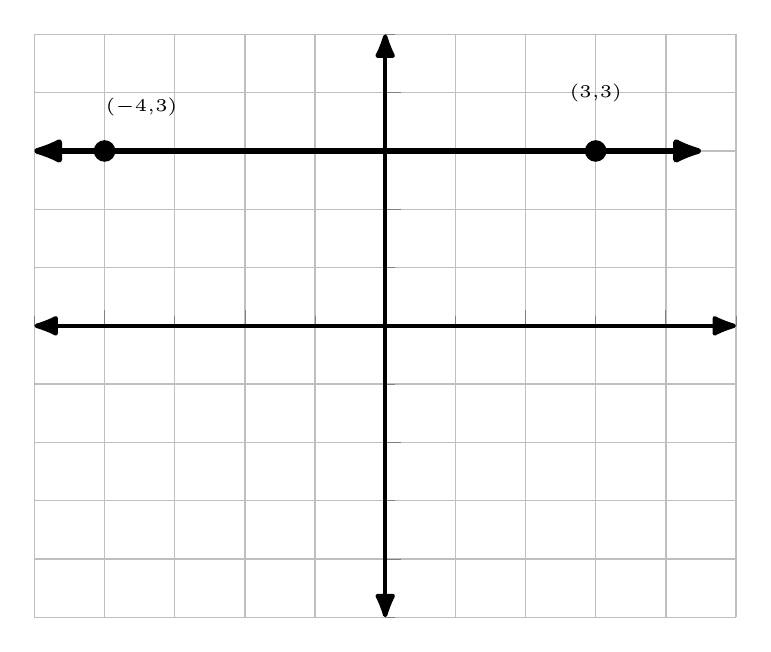
\begin{tikzpicture}[place/.style={circle, fill=black, inner sep=0pt, outer sep=0pt, minimum size=6pt}, scale=1.3
]
\begin{axis} 
[
xticklabels={}, 
yticklabels={}, 
ymin=-5, ymax=5,
xmin=-5, xmax=5,
axis lines = center, 
inner axis line style={Latex[round]-Latex[round],very thick}, 
grid=both,
minor tick num=1, 
%xlabel=$\scriptstyle x$,
%ylabel=$\scriptstyle y$, 
tick align=inside,  
%every axis y label/.style={rotate=0, black, at={(0.5,1.05)},}, 
%every axis x label/.style={rotate=0, black, at={(1.05,0.5)},}, 
%domain=-4.5:4.5, 
%samples=200,
] 

\addplot[<->, >={Latex[round]}, ultra thick, domain=-5:4.5, samples=200]{3}node[]{};

\node (A) at (-4,3) [place] {}; 
\node(A-label) at ($(A)+(50:16pt)$) {$ \scriptscriptstyle (-4,3)$};

\node (B) at (3,3) [place] {}; 
\node(B-label) at ($(B)+(90:16pt)$) {$ \scriptscriptstyle (3,3)$};

\end{axis} 
\end{tikzpicture} 
  
\vspce 
\item \hspce 
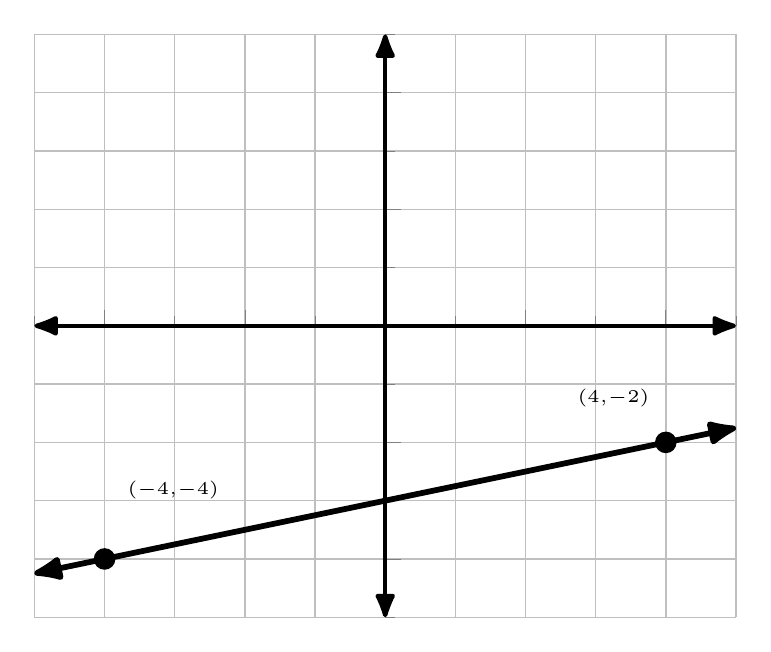
\begin{tikzpicture}[place/.style={circle, fill=black, inner sep=0pt, outer sep=0pt, minimum size=6pt}, scale=1.3
]
\begin{axis} 
[
xticklabels={}, 
yticklabels={}, 
ymin=-5, ymax=5,
xmin=-5, xmax=5,
axis lines = center, 
inner axis line style={Latex[round]-Latex[round],very thick}, 
grid=both,
minor tick num=1, 
%xlabel=$\scriptstyle x$,
%ylabel=$\scriptstyle y$, 
tick align=inside,  
%every axis y label/.style={rotate=0, black, at={(0.5,1.05)},}, 
%every axis x label/.style={rotate=0, black, at={(1.05,0.5)},}, 
%domain=-4.5:4.5, 
%samples=200,
] 

\addplot[<->, >={Latex[round]}, ultra thick, domain=-5:5, samples=200]{x/4-3}node[]{};

\node (A) at (-4,-4) [place] {}; 
\node(A-label) at ($(A)+(45:27pt)$) {$ \scriptscriptstyle (-4,-4)$};

\node (B) at (4,-2) [place] {}; 
\node(B-label) at ($(B)+(140:19pt)$) {$ \scriptscriptstyle (4,-2)$};

\end{axis} 
\end{tikzpicture} 
  
\vspce 
\item \hspce 
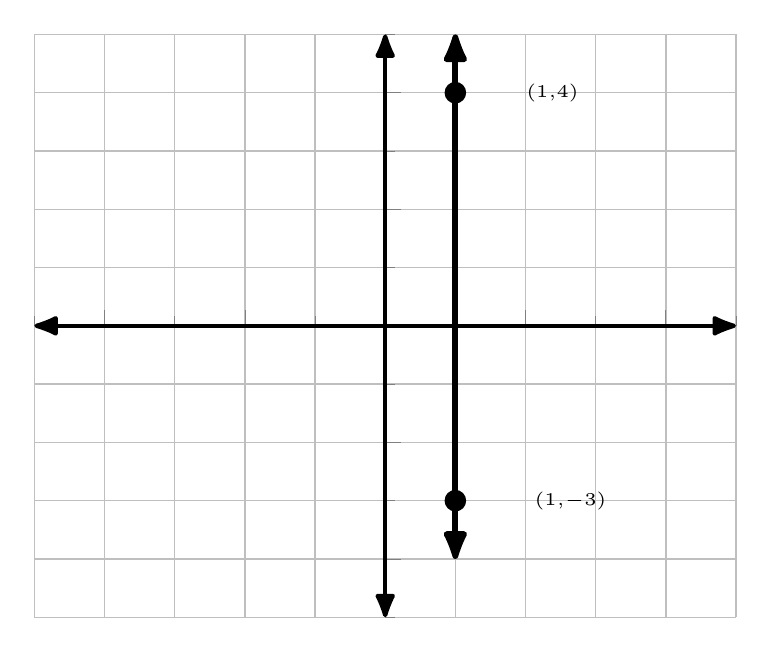
\begin{tikzpicture}[place/.style={circle, fill=black, inner sep=0pt, outer sep=0pt, minimum size=6pt}, scale=1.3
]
\begin{axis} 
[
xticklabels={}, 
yticklabels={}, 
ymin=-5, ymax=5,
xmin=-5, xmax=5,
axis lines = center, 
inner axis line style={Latex[round]-Latex[round],very thick}, 
grid=both,
minor tick num=1, 
%xlabel=$\scriptstyle x$,
%ylabel=$\scriptstyle y$, 
tick align=inside,  
%every axis y label/.style={rotate=0, black, at={(0.5,1.05)},}, 
%every axis x label/.style={rotate=0, black, at={(1.05,0.5)},}, 
%domain=-4.5:4.5, 
%samples=200,
] 

%\addplot[<->, ultra thick, domain=-2.25:0.5, samples=200]{(7/2)*x+3}node[]{};

\node (A) at (1, -3) [place] {}; 
\node(A-label) at ($(A)+(0:32pt)$) {$ \scriptscriptstyle (1, -3)$};

\node (B) at (1, 4) [place] {}; 
\node(B-label) at ($(B)+(0:27pt)$) {$ \scriptscriptstyle (1, 4)$};
\draw[<->, >={Latex[round]}, ultra thick] (1,5) -- (1,-4); 

\end{axis} 
\end{tikzpicture} 
 
\end{multicols} 
\end{enumerate}   

\item  Determine  the slope and trend  of each  line. 

\begin{enumerate}[label = \arabic*. ]
%begin{multicols}{2}

\item \hspce $\ { f(x)=-3x  + 7}$ 
\vspce 
\item \hspce $\ { f(x)=\displaystyle  \frac{1}{4}x-8}$ 
\vspce 
\item \hspce $\ {2x  -  y  = 5 }$ 
\vspce 
\item \hspce $\ { \displaystyle  \frac{1}{2}x+\displaystyle  \frac{1}{4}y-8 = 0 }$ 
\vspce 
\item \hspce $\ {2y  + 1 = 0 }$ 

%end{multicols} 
\end{enumerate}  

\end{enumerate}  

\end{frame}

\end{document}

